\RequirePackage[l2tabu,orthodox]{nag} % Раскомментировав, можно в логе получать рекомендации относительно правильного использования пакетов и предупреждения об устаревших и нерекомендуемых пакетах
% Формат А4, 14pt (ГОСТ Р 7.0.11-2011, 5.3.6)
\documentclass[a4paper,14pt]{extreport}

%%% Проверка используемого TeX-движка %%%
\usepackage{iftex}[2013/04/04]
\newif\ifxetexorluatex   % определяем новый условный оператор (http://tex.stackexchange.com/a/47579/79756)
\ifXeTeX
    \xetexorluatextrue
\else
    \ifLuaTeX
        \xetexorluatextrue
    \else
        \xetexorluatexfalse
    \fi
\fi

%%% Поля и разметка страницы %%%
\usepackage{pdflscape}                              % Для включения альбомных страниц
\usepackage{geometry}                               % Для последующего задания полей

%%% Математические пакеты %%%
\usepackage{amsthm,amsfonts,amsmath,amssymb,amscd}  % Математические дополнения от AMS
\usepackage{mathtools}                              % Добавляет окружение multlined

%%%% Установки для размера шрифта 14 pt %%%%
%% Формирование переменных и констант для сравнения (один раз для всех подключаемых файлов)%%
%% должно располагаться до вызова пакета fontspec или polyglossia, потому что они сбивают его работу
\newlength{\curtextsize}
\newlength{\bigtextsize}
\setlength{\bigtextsize}{13.9pt}

\makeatletter
%\show\f@size                                       % неплохо для отслеживания, но вызывает стопорение процесса, если документ компилируется без команды  -interaction=nonstopmode 
\setlength{\curtextsize}{\f@size pt}
\makeatother

%%% Кодировки и шрифты %%%
\ifxetexorluatex
    \usepackage{polyglossia}[2014/05/21]            % Поддержка многоязычности (fontspec подгружается автоматически)
\else
    \RequirePDFTeX                                  % tests for PDFTEX use and throws an error if a different engine is being used
   %%% Решение проблемы копирования текста в буфер кракозябрами
%    \input glyphtounicode.tex
%    \input glyphtounicode-cmr.tex %from pdfx package
%    \pdfgentounicode=1
    \usepackage{cmap}                               % Улучшенный поиск русских слов в полученном pdf-файле
    \defaulthyphenchar=127                          % Если стоит до fontenc, то переносы не впишутся в выделяемый текст при копировании его в буфер обмена
    \usepackage[T2A]{fontenc}                       % Поддержка русских букв
    \usepackage[utf8]{inputenc}[2014/04/30]         % Кодировка utf8
    \usepackage[english, russian]{babel}[2014/03/24]% Языки: русский, английский
    \IfFileExists{pscyr.sty}{\usepackage{pscyr}}{}  % Красивые русские шрифты
\fi

%%% Оформление абзацев %%%
\usepackage{indentfirst}                            % Красная строка

%%% Цвета %%%
\usepackage[dvipsnames,usenames]{color}
\usepackage{colortbl}
%\usepackage[dvipsnames, table, hyperref, cmyk]{xcolor} % Вероятно, более новый вариант, вместо предыдущих двух строк. Конвертация всех цветов в cmyk заложена как удовлетворение возможного требования типографий. Возможно конвертирование и в rgb.

%%% Таблицы %%%
\usepackage{longtable}                              % Длинные таблицы
\usepackage{multirow,makecell,array}                % Улучшенное форматирование таблиц
\usepackage{booktabs}                               % Возможность оформления таблиц в классическом книжном стиле (при правильном использовании не противоречит ГОСТ)

%%% Общее форматирование
\usepackage{soulutf8}                               % Поддержка переносоустойчивых подчёркиваний и зачёркиваний
\usepackage{icomma}                                 % Запятая в десятичных дробях


%%% Гиперссылки %%%
\usepackage{hyperref}[2012/11/06]

%%% Изображения %%%
\usepackage{graphicx}[2014/04/25]                   % Подключаем пакет работы с графикой

%%% Списки %%%
\usepackage{enumitem}

%%% Подписи %%%
\usepackage{caption}[2013/05/02]                    % Для управления подписями (рисунков и таблиц) % Может управлять номерами рисунков и таблиц с caption %Иногда может управлять заголовками в списках рисунков и таблиц
\usepackage{subcaption}[2013/02/03]                 % Работа с подрисунками и подобным

%%% Интервалы %%%
\usepackage[onehalfspacing]{setspace}               % Опция запуска пакета правит не только интервалы в обычном тексте, но и формульные

%%% Счётчики %%%
\usepackage[figure,table]{totalcount}               % Счётчик рисунков и таблиц
\usepackage{totcount}                               % Пакет создания счётчиков на основе последнего номера подсчитываемого элемента (может требовать дважды компилировать документ)
\usepackage{totpages}                               % Счётчик страниц, совместимый с hyperref (ссылается на номер последней страницы). Желательно ставить последним пакетом в преамбуле

%%% Продвинутое управление групповыми ссылками (пока только формулами) %%%
\ifxetexorluatex
    \usepackage{cleveref}                           % cleveref корректно считывает язык из настроек polyglossia
\else
    \usepackage[russian]{cleveref}                  % cleveref имеет сложности со считыванием языка из babel. Такое решение русификации вывода выбрано вместо определения в documentclass из опасности что-то лишнее передать во все остальные пакеты, включая библиографию.
\fi
\creflabelformat{equation}{#2#1#3}                  % Формат по умолчанию ставил круглые скобки вокруг каждого номера ссылки, теперь просто номера ссылок без какого-либо дополнительного оформления

% \DeclareUTFcharacter[\UTFencname]{x0404}{\CYRIE}
% \DeclareUTFcharacter[\UTFencname]{x0405}{\CYRDZE}
% \DeclareUTFcharacter[\UTFencname]{x0406}{\CYRII}
% \DeclareUTFcharacter[\UTFencname]{x0407}{\CYRYI}
% \DeclareUTFcharacter[\UTFencname]{x0408}{\CYRJE}
% \DeclareUTFcharacter[\UTFencname]{x0409}{\CYRLJE}
% \DeclareUTFcharacter[\UTFencname]{x040A}{\CYRNJE}
% \DeclareUTFcharacter[\UTFencname]{x040B}{\CYRTSHE}
% \DeclareUTFcharacter[\UTFencname]{x040E}{\CYRUSHRT}
% \DeclareUTFcharacter[\UTFencname]{x040F}{\CYRDZHE}
% \DeclareUTFcharacter[\UTFencname]{x0410}{\CYRA}
% \DeclareUTFcharacter[\UTFencname]{x0411}{\CYRB}
% \DeclareUTFcharacter[\UTFencname]{x0412}{\CYRV}
% \DeclareUTFcharacter[\UTFencname]{x0413}{\CYRG}
% \DeclareUTFcharacter[\UTFencname]{x0414}{\CYRD}
% \DeclareUTFcharacter[\UTFencname]{x0415}{\CYRE}
% \DeclareUTFcharacter[\UTFencname]{x0416}{\CYRZH}
% \DeclareUTFcharacter[\UTFencname]{x0417}{\CYRZ}
% \DeclareUTFcharacter[\UTFencname]{x0418}{\CYRI}
% \DeclareUTFcharacter[\UTFencname]{x0419}{\CYRISHRT}
% \DeclareUTFcharacter[\UTFencname]{x041A}{\CYRK}
% \DeclareUTFcharacter[\UTFencname]{x041B}{\CYRL}
% \DeclareUTFcharacter[\UTFencname]{x041C}{\CYRM}
% \DeclareUTFcharacter[\UTFencname]{x041D}{\CYRN}
% \DeclareUTFcharacter[\UTFencname]{x041E}{\CYRO}
% \DeclareUTFcharacter[\UTFencname]{x041F}{\CYRP}
% \DeclareUTFcharacter[\UTFencname]{x0420}{\CYRR}
% \DeclareUTFcharacter[\UTFencname]{x0421}{\CYRS}
% \DeclareUTFcharacter[\UTFencname]{x0422}{\CYRT}
% \DeclareUTFcharacter[\UTFencname]{x0423}{\CYRU}
% \DeclareUTFcharacter[\UTFencname]{x0424}{\CYRF}
% \DeclareUTFcharacter[\UTFencname]{x0425}{\CYRH}
% \DeclareUTFcharacter[\UTFencname]{x0426}{\CYRC}
% \DeclareUTFcharacter[\UTFencname]{x0427}{\CYRCH}
% \DeclareUTFcharacter[\UTFencname]{x0428}{\CYRSH}
% \DeclareUTFcharacter[\UTFencname]{x0429}{\CYRSHCH}
% \DeclareUTFcharacter[\UTFencname]{x042A}{\CYRHRDSN}
% \DeclareUTFcharacter[\UTFencname]{x042B}{\CYRERY}
% \DeclareUTFcharacter[\UTFencname]{x042C}{\CYRSFTSN}
% \DeclareUTFcharacter[\UTFencname]{x042D}{\CYREREV}
% \DeclareUTFcharacter[\UTFencname]{x042E}{\CYRYU}
% \DeclareUTFcharacter[\UTFencname]{x042F}{\CYRYA}
% \DeclareUTFcharacter[\UTFencname]{x0430}{\cyra}
% \DeclareUTFcharacter[\UTFencname]{x0431}{\cyrb}
% \DeclareUTFcharacter[\UTFencname]{x0432}{\cyrv}
% \DeclareUTFcharacter[\UTFencname]{x0433}{\cyrg}
% \DeclareUTFcharacter[\UTFencname]{x0434}{\cyrd}
% \DeclareUTFcharacter[\UTFencname]{x0435}{\cyre}
% \DeclareUTFcharacter[\UTFencname]{x0436}{\cyrzh}
% \DeclareUTFcharacter[\UTFencname]{x0437}{\cyrz}
% \DeclareUTFcharacter[\UTFencname]{x0438}{\cyri}
% \DeclareUTFcharacter[\UTFencname]{x0439}{\cyrishrt}
% \DeclareUTFcharacter[\UTFencname]{x043A}{\cyrk}
% \DeclareUTFcharacter[\UTFencname]{x043B}{\cyrl}
% \DeclareUTFcharacter[\UTFencname]{x043C}{\cyrm}
% \DeclareUTFcharacter[\UTFencname]{x043D}{\cyrn}
% \DeclareUTFcharacter[\UTFencname]{x043E}{\cyro}
% \DeclareUTFcharacter[\UTFencname]{x043F}{\cyrp}
% \DeclareUTFcharacter[\UTFencname]{x0440}{\cyrr}
% \DeclareUTFcharacter[\UTFencname]{x0441}{\cyrs}
% \DeclareUTFcharacter[\UTFencname]{x0442}{\cyrt}
% \DeclareUTFcharacter[\UTFencname]{x0443}{\cyru}
% \DeclareUTFcharacter[\UTFencname]{x0444}{\cyrf}
% \DeclareUTFcharacter[\UTFencname]{x0445}{\cyrh}
% \DeclareUTFcharacter[\UTFencname]{x0446}{\cyrc}
% \DeclareUTFcharacter[\UTFencname]{x0447}{\cyrch}
% \DeclareUTFcharacter[\UTFencname]{x0448}{\cyrsh}
% \DeclareUTFcharacter[\UTFencname]{x0449}{\cyrshch}
% \DeclareUTFcharacter[\UTFencname]{x044A}{\cyrhrdsn}
% \DeclareUTFcharacter[\UTFencname]{x044B}{\cyrery}
% \DeclareUTFcharacter[\UTFencname]{x044C}{\cyrsftsn}
% \DeclareUTFcharacter[\UTFencname]{x044D}{\cyrerev}
% \DeclareUTFcharacter[\UTFencname]{x044E}{\cyryu}
% \DeclareUTFcharacter[\UTFencname]{x044F}{\cyrya}
% \DeclareUTFcharacter[\UTFencname]{x0451}{\cyryo}
% \DeclareUTFcharacter[\UTFencname]{x0452}{\cyrdje}
% \DeclareUTFcharacter[\UTFencname]{x0454}{\cyrie}
% \DeclareUTFcharacter[\UTFencname]{x0455}{\cyrdze}
% \DeclareUTFcharacter[\UTFencname]{x0456}{\cyrii}
% \DeclareUTFcharacter[\UTFencname]{x0457}{\cyryi}
% \DeclareUTFcharacter[\UTFencname]{x0458}{\cyrje}
% \DeclareUTFcharacter[\UTFencname]{x0459}{\cyrlje}
% \DeclareUTFcharacter[\UTFencname]{x045A}{\cyrnje}
% \DeclareUTFcharacter[\UTFencname]{x045B}{\cyrtshe}
% \DeclareUTFcharacter[\UTFencname]{x045E}{\cyrushrt}
% \DeclareUTFcharacter[\UTFencname]{x045F}{\cyrdzhe}
% \DeclareUTFcharacter[\UTFencname]{x0490}{\CYRGUP}
% \DeclareUTFcharacter[\UTFencname]{x0491}{\cyrgup}
% \DeclareUTFcharacter[\UTFencname]{x0492}{\CYRGHCRS}
% \DeclareUTFcharacter[\UTFencname]{x0493}{\cyrghcrs}
% \DeclareUTFcharacter[\UTFencname]{x0496}{\CYRZHDSC}
% \DeclareUTFcharacter[\UTFencname]{x0497}{\cyrzhdsc}
% \DeclareUTFcharacter[\UTFencname]{x0498}{\CYRZDSC}
% \DeclareUTFcharacter[\UTFencname]{x0499}{\cyrzdsc}
% \DeclareUTFcharacter[\UTFencname]{x049A}{\CYRKDSC}
% \DeclareUTFcharacter[\UTFencname]{x049B}{\cyrkdsc}
% \DeclareUTFcharacter[\UTFencname]{x049C}{\CYRKVCRS}
% \DeclareUTFcharacter[\UTFencname]{x049D}{\cyrkvcrs}
% \DeclareUTFcharacter[\UTFencname]{x04A0}{\CYRKBEAK}
% \DeclareUTFcharacter[\UTFencname]{x04A1}{\cyrkbeak}
% \DeclareUTFcharacter[\UTFencname]{x04A2}{\CYRNDSC}
% \DeclareUTFcharacter[\UTFencname]{x04A3}{\cyrndsc}
% \DeclareUTFcharacter[\UTFencname]{x04A4}{\CYRNG}
% \DeclareUTFcharacter[\UTFencname]{x04A5}{\cyrng}
% \DeclareUTFcharacter[\UTFencname]{x04AA}{\CYRSDSC}
% \DeclareUTFcharacter[\UTFencname]{x04AB}{\cyrsdsc}
% \DeclareUTFcharacter[\UTFencname]{x04AE}{\CYRY}
% \DeclareUTFcharacter[\UTFencname]{x04AF}{\cyry}
% \DeclareUTFcharacter[\UTFencname]{x04B0}{\CYRYHCRS}
% \DeclareUTFcharacter[\UTFencname]{x04B1}{\cyryhcrs}
% \DeclareUTFcharacter[\UTFencname]{x04B2}{\CYRHDSC}
% \DeclareUTFcharacter[\UTFencname]{x04B3}{\cyrhdsc}
% \DeclareUTFcharacter[\UTFencname]{x04B6}{\CYRCHRDSC}
% \DeclareUTFcharacter[\UTFencname]{x04B7}{\cyrchrdsc}
% \DeclareUTFcharacter[\UTFencname]{x04B8}{\CYRCHVCRS}
% \DeclareUTFcharacter[\UTFencname]{x04B9}{\cyrchvcrs}
% \DeclareUTFcharacter[\UTFencname]{x04BA}{\CYRSHHA}
% \DeclareUTFcharacter[\UTFencname]{x04BB}{\cyrshha}
% \DeclareUTFcharacter[\UTFencname]{x04C0}{\CYRpalochka}
% \DeclareUTFcharacter[\UTFencname]{x04D4}{\CYRAE}
% \DeclareUTFcharacter[\UTFencname]{x04D5}{\cyrae}
% \DeclareUTFcharacter[\UTFencname]{x04D8}{\CYRSCHWA}
% \DeclareUTFcharacter[\UTFencname]{x04D9}{\cyrschwa}

  % Пакеты общие для диссертации и автореферата
%%% Колонтитулы %%%
\usepackage{fancyhdr}

%%% Прикладные пакеты %%% 
\usepackage{calc}               % Пакет для расчётов параметров, например длины
%\usepackage{etoolbox}          % ради функции patchcmd для управления списком литературы

\usepackage {interfaces-base}   % Набор базовых интерфейсов к некоторым пакетам, конкретные реализации загружаются в стиле

%%% Заголовки %%%
\usepackage{titlesec}           % Пакет настройки шрифтов заголовков в тексте

%%% Оглавление %%%
\usepackage{tocloft}

%%% Счётчики %%%
\usepackage{chngcntr}           % оперативная перенастройка счётчиков         % Пакеты для диссертации
\usepackage{tabularx, tabu, tabulary}  %таблицы с автоматически подбирающейся шириной столбцов

% Листинги с исходным кодом программ
\usepackage{fancyvrb}
\usepackage{listings}

% Плавающие окружения. во многом лучше пакета float
\usepackage{floatrow}

% Русская традиция начертания греческих букв
%\usepackage{upgreek} % прямые греческие ради русской традиции

\usepackage[ruled,vlined]{algorithm2e}                          % Описание алгоритмов на псевдокоде
\usepackage{enumitem}

% correct spacing after macros
\usepackage{xspace}

% striked text with \st{}
\usepackage{soul}

% allow hyperref link to the top of related object instead of its caption
\usepackage{caption}

\usepackage{graphicx, epsfig}
\usepackage{color}
\usepackage{xcolor}        % Пакеты для специфических пользовательских задач

%%%%%%%%%%%%%%%%%%%%%%%%%%%%%%%%%%%%%%%%%%%%%%%%%%%%%%
%%%% Файл упрощённых настроек шаблона диссертации %%%%
%%%%%%%%%%%%%%%%%%%%%%%%%%%%%%%%%%%%%%%%%%%%%%%%%%%%%%

%%%        Подключение пакетов                 %%%
\usepackage{ifthen}                 % добавляет ifthenelse
%%% Инициализирование переменных, не трогать!  %%%
\newcounter{bibliosel}
\newcounter{tabcap}
\newcounter{tablaba}
\newcounter{tabtita}
%%%%%%%%%%%%%%%%%%%%%%%%%%%%%%%%%%%%%%%%%%%%%%%%%%

%%% Область упрощённого управления оформлением %%%

%% Библиография

%% Внимание! При использовании bibtex8 необходимо удалить все
%% цитирования из  ../common/characteristic.tex 
\setcounter{bibliosel}{1}           % 0 --- встроенная реализация с загрузкой файла через движок bibtex8; 1 --- реализация пакетом biblatex через движок biber

%% Подпись таблиц
\setcounter{tabcap}{0}              % 0 --- по ГОСТ, номер таблицы и название разделены тире, выровнены по левому краю, при необходимости на нескольких строках; 1 --- подпись таблицы не по ГОСТ, на двух и более строках, дальнейшие настройки: 
%Выравнивание первой строки, с подписью и номером
\setcounter{tablaba}{2}             % 0 --- по левому краю; 1 --- по центру; 2 --- по правому краю
%Выравнивание строк с самим названием таблицы
\setcounter{tabtita}{1}             % 0 --- по левому краю; 1 --- по центру; 2 --- по правому краю

%%% Цвета гиперссылок %%%
% Latex color definitions: http://latexcolor.com/
\definecolor{linkcolor}{rgb}{0.9,0,0}
\definecolor{citecolor}{rgb}{0,0.6,0}
\definecolor{urlcolor}{rgb}{0,0,1}
%\definecolor{linkcolor}{rgb}{0,0,0} %black
%\definecolor{citecolor}{rgb}{0,0,0} %black
%\definecolor{urlcolor}{rgb}{0,0,0} %black               % Упрощённые настройки шаблона

%%% Переопределение именований, чтобы можно было и в преамбуле использовать %%%
\renewcommand{\chaptername}{Глава}
\renewcommand{\appendixname}{Приложение} % (ГОСТ Р 7.0.11-2011, 5.7)
       % Переопределение именований, чтобы можно было и в преамбуле использовать
% Новые переменные, которые могут использоваться во всём проекте
\newcommand{\authorbibtitle}{Публикации автора по теме диссертации}
\newcommand{\fullbibtitle}{Список литературы} % (ГОСТ Р 7.0.11-2011, 4)

% I fucking cannot format this 'if' properly because
% of fucking spacing issues
\newcommand{\CH}[1][]{\ifthenelse{ \equal{#1}{*} }
        {\texttt{CascadeHeap*}}
        {\ifthenelse{ \equal{#1}{} }
            {\texttt{CascadeHeap}}
            {\texttt{CascadeHeap[#1]}}}\xspace}

\newcommand{\SCH}{\texttt{SimpleCascadeHeap}\xspace}
\newcommand{\myB}{\texttt{B}\xspace}
\newcommand{\MH}[1][]{\ifthenelse{ \equal{#1}{} }
        {\texttt{MH}}
        {\texttt{MH$_{#1}$}}\xspace}
\newcommand{\HH}{\texttt{HH}\xspace}

\newcommand{\PartSort}{\texttt{PartialSorting}\xspace}
\newcommand{\IncSort}{\texttt{IncrementalSorting}\xspace}
\newcommand{\PriQ}{\texttt{PriorityQueue}\xspace}

% Theorems
\newtheorem*{theorem-star}{Теорема}
\newtheorem{theorem}{Теорема}[section]
\newtheorem*{theorem-definition-star}{Теорема-определение}
\newtheorem*{corollary-star}{Следствие}
\newtheorem{corollary}{Следствие}[section]
\newtheorem*{property-star}{Свойство}
\newtheorem*{properties}{Свойства}
\newtheorem{property}{Свойство}
\newtheorem*{lem-star}{Лемма}
\newtheorem{lem}{Лемма}[section]
\newtheorem*{proposition-star}{Предложение}
\newtheorem{proposition}{Предложение}
\newtheorem{stage}{Этап}
\newtheorem*{statement}{Утверждение}
\newtheorem*{usage}{Использование}

\theoremstyle{remark}
\newtheorem*{remark}{Замечание}

\theoremstyle{definition}
\newtheorem{problem}{Задача}
\newtheorem{exercise}{Упражнение}

\theoremstyle{definition}
\newtheorem*{definition-star}{Определение}
\newtheorem{definition}{Определение}[section]
\newtheorem*{designation}{Обозначение}

\theoremstyle{definition}
\newtheorem*{example-star}{Пример}
\newtheorem{example}{Пример}
\newtheorem*{examples}{Примеры}
\newtheorem{case}{Случай}
\newtheorem*{case-star}{Случай}

\newcommand{\myX}{\mathcal{X}}
\newcommand{\myH}{\mathcal{H}}

\DeclareMathOperator{\lev}{level}

% algorihtm2e stuff
\newcommand{\DefineAlgoKeywords}{
\SetKwArray{BalState}{BalancingState}
\SetKwArray{T}{T}
\SetKwData{BufSize}{BufferSize}
\SetKwData{C}{C}
\SetKwData{ElemCount}{InsertionsCount}
\SetKwData{NoAction}{NoAction}
\SetKwData{StateI}{State1}
\SetKwData{StateII}{State2}
\SetKwData{x}{x}
\SetKwData{MaxLevel}{MaximumLevel}
}
\newcommand{\Gets}{\ $\gets$\ }

  % Новые переменные, которые могут использоваться во всём проекте

%%% Основные сведения %%%
\newcommand{\thesisAuthor}             % Диссертация, ФИО автора
{%
    \texorpdfstring{% \texorpdfstring takes two arguments and uses the first for (La)TeX and the second for pdf
        Иванов Илья Сергеевич% так будет отображаться на титульном листе или в тексте, где будет использоваться переменная
    }{%
        Иванов, Илья Сергеевич% эта запись для свойств pdf-файла. В таком виде, если pdf будет обработан программами для сбора библиографических сведений, будет правильно представлена фамилия.
    }%
}
\newcommand{\thesisAuthorShort}             % Диссертация, ФИО автора инициалами
{Иванов И. С.}

\newcommand{\MyThesisTitle}{Рекуррентные нейронные сети с механизмом внимания для анализа тональности русских текстов}

\newcommand{\thesisUdk}                % Диссертация, УДК
{\todo{xxx.xxx}}
\newcommand{\thesisTitle}              % Диссертация, название
{\texorpdfstring{\MakeUppercase{\MyThesisTitle}}{\MyThesisTitle}}
\newcommand{\thesisSpecialtyNumber}    % Диссертация, специальность, номер
{\texorpdfstring{\todo{XX.XX.XX}}{XX.XX.XX}}
\newcommand{\thesisSpecialtyTitle}     % Диссертация, специальность, название
{\texorpdfstring{\todo{Название специальности}}{Название специальности}}
\newcommand{\thesisDegree}             % Диссертация, научная степень
{\todo{кандидата физико-математических наук}}
\newcommand{\thesisCity}               % Диссертация, город защиты
{МОСКВА}
\newcommand{\thesisYear}               % Диссертация, год защиты
{2017}
\newcommand{\thesisOrganization}       % Диссертация, организация
{Московский физико-технический институт (государственный университет)}

\newcommand{\thesisOrganizationShort}  % Диссертация, краткое название организации для доклада
{\todo{НазУчДисРаб}}

\newcommand{\thesisInOrganization}       % Диссертация, организация в предложном падеже: Работа выполнена в ...
{Московском физико-техническом институте (государственном университете)}

\newcommand{\supervisorFio}            % Научный руководитель, ФИО
{Бурцев Михаил Сергеевич}
\newcommand{\supervisorRegalia}        % Научный руководитель, регалии
{\todo{уч. степень, уч. звание}}
\newcommand{\supervisorFioShort}            % Научный руководитель, ФИО
{М.~С.~Бурцев}
\newcommand{\supervisorRegaliaShort}        % Научный руководитель, регалии
{\todo{уч.~ст.,~уч.~зв.}}


\newcommand{\opponentOneFio}           % Оппонент 1, ФИО
{\todo{Фамилия Имя Отчество}}
\newcommand{\opponentOneRegalia}       % Оппонент 1, регалии
{\todo{доктор физико-математических наук, профессор}}
\newcommand{\opponentOneJobPlace}      % Оппонент 1, место работы
{\todo{Не очень длинное название для места работы}}
\newcommand{\opponentOneJobPost}       % Оппонент 1, должность
{\todo{старший научный сотрудник}}

\newcommand{\opponentTwoFio}           % Оппонент 2, ФИО
{\todo{Фамилия Имя Отчество}}
\newcommand{\opponentTwoRegalia}       % Оппонент 2, регалии
{\todo{кандидат физико-математических наук}}
\newcommand{\opponentTwoJobPlace}      % Оппонент 2, место работы
{\todo{Основное место работы c длинным длинным длинным длинным названием}}
\newcommand{\opponentTwoJobPost}       % Оппонент 2, должность
{\todo{старший научный сотрудник}}

\newcommand{\leadingOrganizationTitle} % Ведущая организация, дополнительные строки
{\todo{Федеральное государственное бюджетное образовательное учреждение высшего профессионального образования с~длинным длинным длинным длинным названием}}

\newcommand{\defenseDate}              % Защита, дата
{\todo{DD mmmmmmmm YYYY~г.~в~XX часов}}
\newcommand{\defenseCouncilNumber}     % Защита, номер диссертационного совета
{\todo{NN}}
\newcommand{\defenseCouncilTitle}      % Защита, учреждение диссертационного совета
{\todo{Название учреждения}}
\newcommand{\defenseCouncilAddress}    % Защита, адрес учреждение диссертационного совета
{\todo{Адрес}}

\newcommand{\defenseSecretaryFio}      % Секретарь диссертационного совета, ФИО
{\todo{Фамилия Имя Отчество}}
\newcommand{\defenseSecretaryRegalia}  % Секретарь диссертационного совета, регалии
{\todo{д-р~физ.-мат. наук}}            % Для сокращений есть ГОСТы, например: ГОСТ Р 7.0.12-2011 + http://base.garant.ru/179724/#block_30000

\newcommand{\synopsisLibrary}          % Автореферат, название библиотеки
{\todo{Название библиотеки}}
\newcommand{\synopsisDate}             % Автореферат, дата рассылки
{\todo{DD mmmmmmmm YYYY года}}

% To avoid conflict with beamer class use \providecommand
\providecommand{\keywords}%                 % Ключевые слова для метаданных PDF диссертации и автореферата
{}
      % Основные сведения
%%% Макет страницы %%%
% Выставляем значения полей (ГОСТ 7.0.11-2011, 5.3.7)
\geometry{a4paper,top=2cm,bottom=2cm,left=3cm,right=2cm}

%%% Кодировки и шрифты %%%
\ifxetexorluatex
    \setmainlanguage[babelshorthands=true]{russian}  % Язык по-умолчанию русский с поддержкой приятных команд пакета babel
    \setotherlanguage{english}                       % Дополнительный язык = английский (в американской вариации по-умолчанию)
    \setmonofont{Courier New}
    \newfontfamily\cyrillicfonttt{Courier New}
    \ifXeTeX
        \defaultfontfeatures{Ligatures=TeX,Mapping=tex-text}
    \else
        \defaultfontfeatures{Ligatures=TeX}
    \fi
    \setmainfont{Times New Roman}
    \newfontfamily\cyrillicfont{Times New Roman}
    \setsansfont{Arial}
    \newfontfamily\cyrillicfontsf{Arial}
\else
    \IfFileExists{pscyr.sty}{\renewcommand{\rmdefault}{ftm}}{}
\fi

%%% Интервалы %%%
%linespread-реализация ближе к реализации полуторного интервала в ворде.
%setspace реализация заточена под шрифты 10, 11, 12pt, под остальные кегли хуже, но всё же ближе к типографской классике. 
%\linespread{1.42}                    % Полуторный интервал (ГОСТ Р 7.0.11-2011, 5.3.6)

%%% Выравнивание и переносы %%%
\sloppy                             % Избавляемся от переполнений
\clubpenalty=10000                  % Запрещаем разрыв страницы после первой строки абзаца
\widowpenalty=10000                 % Запрещаем разрыв страницы после последней строки абзаца

%%% Подписи %%%
\captionsetup{%
singlelinecheck=off,                % Многострочные подписи, например у таблиц
skip=2pt,                           % Вертикальная отбивка между подписью и содержимым рисунка или таблицы определяется ключом
justification=centering,            % Центрирование подписей, заданных командой \caption
}

%%% Рисунки %%%
\DeclareCaptionLabelSeparator*{emdash}{~--- }             % (ГОСТ 2.105, 4.3.1)
\captionsetup[figure]{labelsep=emdash,font=onehalfspacing,position=bottom}

%%% Таблицы %%%
\ifthenelse{\equal{\thetabcap}{0}}{%
    \newcommand{\tabcapalign}{\raggedright}  % по левому краю страницы или аналога parbox
}

\ifthenelse{\equal{\thetablaba}{0} \AND \equal{\thetabcap}{1}}{%
    \newcommand{\tabcapalign}{\raggedright}  % по левому краю страницы или аналога parbox
}

\ifthenelse{\equal{\thetablaba}{1} \AND \equal{\thetabcap}{1}}{%
    \newcommand{\tabcapalign}{\centering}    % по центру страницы или аналога parbox
}

\ifthenelse{\equal{\thetablaba}{2} \AND \equal{\thetabcap}{1}}{%
    \newcommand{\tabcapalign}{\raggedleft}   % по правому краю страницы или аналога parbox
}

\ifthenelse{\equal{\thetabtita}{0} \AND \equal{\thetabcap}{1}}{%
    \newcommand{\tabtitalign}{\raggedright}  % по левому краю страницы или аналога parbox
}

\ifthenelse{\equal{\thetabtita}{1} \AND \equal{\thetabcap}{1}}{%
    \newcommand{\tabtitalign}{\centering}    % по центру страницы или аналога parbox
}

\ifthenelse{\equal{\thetabtita}{2} \AND \equal{\thetabcap}{1}}{%
    \newcommand{\tabtitalign}{\raggedleft}   % по правому краю страницы или аналога parbox
}

\DeclareCaptionFormat{tablenocaption}{\tabcapalign #1\strut}        % Наименование таблицы отсутствует
\ifthenelse{\equal{\thetabcap}{0}}{%
    \DeclareCaptionFormat{tablecaption}{\tabcapalign #1#2#3}
    \captionsetup[table]{labelsep=emdash}                       % тире как разделитель идентификатора с номером от наименования
}{%
    \DeclareCaptionFormat{tablecaption}{\tabcapalign #1#2\par%  % Идентификатор таблицы на отдельной строке
        \tabtitalign{#3}}                                       % Наименование таблицы строкой ниже
    \captionsetup[table]{labelsep=space}                        % пробельный разделитель идентификатора с номером от наименования
}
\captionsetup[table]{format=tablecaption,singlelinecheck=off,font=onehalfspacing,position=top,skip=0pt}  % многострочные наименования и прочее
\DeclareCaptionLabelFormat{continued}{Продолжение таблицы~#2}

%%% Подписи подрисунков %%%
\renewcommand{\thesubfigure}{\asbuk{subfigure}}           % Буквенные номера подрисунков
\captionsetup[subfigure]{font={normalsize},               % Шрифт подписи названий подрисунков (не отличается от основного)
    labelformat=brace,                                    % Формат обозначения подрисунка
    justification=centering,                              % Выключка подписей (форматирование), один из вариантов            
}
%\DeclareCaptionFont{font12pt}{\fontsize{12pt}{13pt}\selectfont} % объявляем шрифт 12pt для использования в подписях, тут же надо интерлиньяж объявлять, если не наследуется
%\captionsetup[subfigure]{font={font12pt}}                 % Шрифт подписи названий подрисунков (всегда 12pt)

%%% Настройки гиперссылок %%%
\ifLuaTeX
    \hypersetup{
        unicode,                % Unicode encoded PDF strings
    }
\fi

\hypersetup{
    linktocpage=true,           % ссылки с номера страницы в оглавлении, списке таблиц и списке рисунков
%    linktoc=all,                % both the section and page part are links
%    pdfpagelabels=false,        % set PDF page labels (true|false)
    plainpages=false,           % Forces page anchors to be named by the Arabic form  of the page number, rather than the formatted form
    colorlinks,                 % ссылки отображаются раскрашенным текстом, а не раскрашенным прямоугольником, вокруг текста
    linkcolor={linkcolor},      % цвет ссылок типа ref, eqref и подобных
    citecolor={citecolor},      % цвет ссылок-цитат
    urlcolor={urlcolor},        % цвет гиперссылок
%    hidelinks,                  % Hide links (removing color and border)
    pdftitle={\thesisTitle},    % Заголовок
    pdfauthor={\thesisAuthor},  % Автор
    pdfsubject={\thesisSpecialtyNumber\ \thesisSpecialtyTitle},      % Тема
%    pdfcreator={Создатель},     % Создатель, Приложение
%    pdfproducer={Производитель},% Производитель, Производитель PDF
    pdfkeywords={\keywords},    % Ключевые слова
    pdflang={ru},
}

%%% Шаблон %%%
\DeclareRobustCommand{\todo}{\textcolor{red}}       % решаем проблему превращения названия цвета в результате \MakeUppercase, http://tex.stackexchange.com/a/187930/79756 , \DeclareRobustCommand protects \todo from expanding inside \MakeUppercase
\setlength{\parindent}{2.5em}                       % Абзацный отступ. Должен быть одинаковым по всему тексту и равен пяти знакам (ГОСТ Р 7.0.11-2011, 5.3.7).

%%% Списки %%%
% Используем короткое тире (endash) для ненумерованных списков (ГОСТ 2.105-95, пункт 4.1.7, требует дефиса, но так лучше смотрится)
\renewcommand{\labelitemi}{\normalfont\bfseries{--}}

% Перечисление строчными буквами латинского алфавита (ГОСТ 2.105-95, 4.1.7)
%\renewcommand{\theenumi}{\alph{enumi}}
%\renewcommand{\labelenumi}{\theenumi)} 

% Перечисление строчными буквами русского алфавита (ГОСТ 2.105-95, 4.1.7)
%\makeatletter
%\AddEnumerateCounter{\asbuk}{\russian@alph}{щ}      % Управляем списками/перечислениями через пакет enumitem, а он 'не знает' про asbuk, потому 'учим' его
%\makeatother
%\renewcommand{\theenumi}{\asbuk{enumi}}
%\renewcommand{\labelenumi}{\theenumi)} 

\setlist{nosep,%                                    % Единый стиль для всех списков (пакет enumitem), без дополнительных интервалов.
    labelindent=\parindent,leftmargin=*%            % Каждый пункт, подпункт и перечисление записывают с абзацного отступа (ГОСТ 2.105-95, 4.1.8)
}
    % Стили общие для диссертации и автореферата
%%% Изображения %%%
\graphicspath{{images/}{Dissertation/images/}}         % Пути к изображениям

\LoadInterface {titlesec}                   % Подгружаем интерфейсы для дополнительных опций управления некоторыми пакетами

%%% Блок управления параметрами для выравнивания заголовков в тексте %%%
\newlength{\otstuplen}
\setlength{\otstuplen}{\theotstup\parindent}
\ifthenelse{\equal{\theheadingalign}{0}}{% выравнивание заголовков в тексте
    \newcommand{\hdngalign}{\filcenter}                % по центру
    \newcommand{\hdngaligni}{\hfill\hspace{\otstuplen}}% по центру
}{%
    \newcommand{\hdngalign}{\filright}                 % по левому краю
    \newcommand{\hdngaligni}{\hspace{\otstuplen}}      % по левому краю
} % В обоих случаях вроде бы без переноса, как и надо (ГОСТ Р 7.0.11-2011, 5.3.5)

%%% Оглавление %%%
\renewcommand{\cftchapdotsep}{\cftdotsep}                % отбивка точками до номера страницы начала главы/раздела
\renewcommand{\cfttoctitlefont}{\hdngaligni\fontsize{14pt}{16pt}\selectfont\bfseries}% вместе со следующей строкой
\renewcommand{\cftaftertoctitle}{\hfill}                 % устанавливает заголовок по центру
\setlength{\cftbeforetoctitleskip}{-1.4\curtextsize}     % Поскольку этот заголовок всегда является первым на странице, то перед ним отделять пустым тройным интервалом не следует. Независимо от основного шрифта, в этом случае зануление (почти) происходит при -1.4\curtextsize.
\setlength{\cftaftertoctitleskip}{\theintvl\curtextsize} % Если считаем Оглавление заголовком, то выставляем после него тройной интервал через наше определённое значение

%% Переносить слова в заголовке не допускается (ГОСТ Р 7.0.11-2011, 5.3.5). Заголовки в оглавлении должны точно повторять заголовки в тексте (ГОСТ Р 7.0.11-2011, 5.2.3). Прямого указания на запрет переносов в оглавлении нет, но по той же логике невнесения искажений в смысл, лучше в оглавлении не переносить:
\cftsetrmarg{2.55em plus1fil}                       %To have the (sectional) titles in the ToC, etc., typeset ragged right with no hyphenation
\renewcommand{\cftchappagefont}{\normalfont}        % нежирные номера страниц у глав в оглавлении
\renewcommand{\cftchapleader}{\cftdotfill{\cftchapdotsep}}% нежирные точки до номеров страниц у глав в оглавлении
%\renewcommand{\cftchapfont}{}                       % нежирные названия глав в оглавлении

\ifthenelse{\theheadingdelim > 0}{%
    \renewcommand\cftchapaftersnum{.\ }   % добавляет точку с пробелом после номера раздела в оглавлении
}{%
\renewcommand\cftchapaftersnum{\quad}     % добавляет \quad после номера раздела в оглавлении
}
\ifthenelse{\theheadingdelim > 1}{%
    \renewcommand\cftsecaftersnum{.\ }    % добавляет точку с пробелом после номера подраздела в оглавлении
    \renewcommand\cftsubsecaftersnum{.\ } % добавляет точку с пробелом после номера подподраздела в оглавлении
}{%
\renewcommand\cftsecaftersnum{\quad}      % добавляет \quad после номера подраздела в оглавлении
\renewcommand\cftsubsecaftersnum{\quad}   % добавляет \quad после номера подподраздела в оглавлении
}

\ifthenelse{\equal{\thepgnum}{1}}{%
    \addtocontents{toc}{~\hfill{Стр.}\par}% добавить Стр. над номерами страниц
}

%%% Оформление названий глав %%%
%% настройки заголовка списка рисунков
\renewcommand{\cftloftitlefont}{\hdngaligni\fontsize{14pt}{16pt}\selectfont\bfseries}% вместе со следующей строкой
\renewcommand{\cftafterloftitle}{\hfill}                                             % устанавливает заголовок по центру
\setlength{\cftbeforeloftitleskip}{-1.5\curtextsize}     % Поскольку этот заголовок всегда является первым на странице, то перед ним отделять пустым тройным интервалом не следует. Независимо от основного шрифта, в этом случае зануление (почти) происходит при -1.5\curtextsize.
\setlength{\cftafterloftitleskip}{\theintvl\curtextsize} % выставляем после него тройной интервал через наше определённое значение

%% настройки заголовка списка таблиц
\renewcommand{\cftlottitlefont}{\hdngaligni\fontsize{14pt}{16pt}\selectfont\bfseries}% вместе со следующей строкой
\renewcommand{\cftafterlottitle}{\hfill}                                             % устанавливает заголовок по центру
\setlength{\cftbeforelottitleskip}{-1.5\curtextsize}     % Поскольку этот заголовок всегда является первым на странице, то перед ним отделять пустым тройным интервалом не следует. Независимо от основного шрифта, в этом случае зануление (почти) происходит при -1.5\curtextsize.
\setlength{\cftafterlottitleskip}{\theintvl\curtextsize} % выставляем после него тройной интервал через наше определённое значение

\ifnum\curtextsize>\bigtextsize     % Проверяем условие использования базового шрифта 14 pt
\setlength{\headheight}{17pt}       % Исправляем высоту заголовка
\else
\setlength{\headheight}{15pt}       % Исправляем высоту заголовка
\fi

%%% Колонтитулы %%%
% Порядковый номер страницы печатают на середине верхнего поля страницы (ГОСТ Р 7.0.11-2011, 5.3.8)
\makeatletter
\let\ps@plain\ps@fancy              % Подчиняем первые страницы каждой главы общим правилам
\makeatother
\pagestyle{fancy}                   % Меняем стиль оформления страниц
\fancyhf{}                          % Очищаем текущие значения
\fancyhead[C]{\thepage}             % Печатаем номер страницы на середине верхнего поля
\renewcommand{\headrulewidth}{0pt}  % Убираем разделительную линию

%%% Оформление заголовков глав, разделов, подразделов %%%
%% Работа должна быть выполнена ... размером шрифта 12-14 пунктов (ГОСТ Р 7.0.11-2011, 5.3.8). То есть не должно быть надписей шрифтом более 14. Так и поставим.
%% Эти установки будут давать одинаковый результат независимо от выбора базовым шрифтом 12 пт или 14 пт
\titleformat{\chapter}[block]                                % default display;  hang = with a hanging label. (Like the standard \section.); block = typesets the whole title in a block (a paragraph) without additional formatting. Useful in centered titles
        {\hdngalign\fontsize{14pt}{16pt}\selectfont\bfseries}% 
        %\fontsize{<size>}{<skip>} % второе число ставим 1.2*первое, чтобы адекватно отрабатывали команды по расчету полуторного интервала (домножая разные комбинации коэффициентов на этот)
        {\thechapter\cftchapaftersnum}                       % Заголовки в оглавлении должны точно повторять заголовки в тексте (ГОСТ Р 7.0.11-2011, 5.2.3).
        {0em}% отступ от номера до текста
        {}%

\titleformat{\section}[block]                                % default hang;  hang = with a hanging label. (Like the standard \section.); block = typesets the whole title in a block (a paragraph) without additional formatting. Useful in centered titles
        {\hdngalign\fontsize{14pt}{16pt}\selectfont\bfseries}% 
        %\fontsize{<size>}{<skip>} % второе число ставим 1.2*первое, чтобы адекватно отрабатывали команды по расчету полуторного интервала (домножая разные комбинации коэффициентов на этот)
        {\thesection\cftsecaftersnum}                        % Заголовки в оглавлении должны точно повторять заголовки в тексте (ГОСТ Р 7.0.11-2011, 5.2.3).
        {0em}% отступ от номера до текста
        {}%

\titleformat{\subsection}[block]                             % default hang;  hang = with a hanging label. (Like the standard \section.); block = typesets the whole title in a block (a paragraph) without additional formatting. Useful in centered titles
        {\hdngalign\fontsize{14pt}{16pt}\selectfont\bfseries}% 
        %\fontsize{<size>}{<skip>} % второе число ставим 1.2*первое, чтобы адекватно отрабатывали команды по расчету полуторного интервала (домножая разные комбинации коэффициентов на этот)
        {\thesubsection\cftsubsecaftersnum}                  % Заголовки в оглавлении должны точно повторять заголовки в тексте (ГОСТ Р 7.0.11-2011, 5.2.3).
        {0em}% отступ от номера до текста
        {}%

\ifthenelse{\equal{\thechapstyle}{1}}{%
    \sectionformat{\chapter}{% Параметры заголовков разделов в тексте
        label=\chaptername\ \thechapter\cftchapaftersnum,
        labelsep=0em,
    }
    %% Следующие две строки: будет вписано слово Глава перед каждым номером раздела в оглавлении   
    \renewcommand{\cftchappresnum}{\chaptername\ }
    \setlength{\cftchapnumwidth}{\widthof{\cftchapfont\cftchappresnum\thechapter\cftchapaftersnum}}
}%

%% Интервалы между заголовками
% На эти величины titlespacing множит через *
\beforetitleunit=\curtextsize% привязались к нашему размеру шрифта
\aftertitleunit=\curtextsize% привязались к нашему размеру шрифта

% Счётчик intvl и длина \otstup определены в файле setup
\titlespacing{\chapter}{\theotstup\parindent}{-1.7em}{*\theintvl}       % Заголовки отделяют от текста сверху и снизу тремя интервалами (ГОСТ Р 7.0.11-2011, 5.3.5). Поскольку название главы всегда является первым на странице, то перед ним отделять пустым тройным интервалом не следует. Независимо от основного шрифта, в этом случае зануление происходит при -1.7em.
\titlespacing{\section}{\theotstup\parindent}{*\theintvl}{*\theintvl}
\titlespacing{\subsection}{\theotstup\parindent}{*\theintvl}{*\theintvl}
\titlespacing{\subsubsection}{\theotstup\parindent}{*\theintvl}{*\theintvl}

%%% Блок дополнительного управления размерами заголовков
\ifthenelse{\equal{\theheadingsize}{1}}{% Пропорциональные заголовки и базовый шрифт 14 пт
    \renewcommand{\cfttoctitlefont}{\hdngaligni\Large\bfseries} % Исправляем размер заголовка оглавления
    \setlength{\cftbeforetoctitleskip}{-1.2\curtextsize}        % Исправляем вертикальный отступ перед заголовком оглавления
    \renewcommand{\cftloftitlefont}{\hdngaligni\Large\bfseries} % Исправляем размер заголовка списка рисунков
    \setlength{\cftbeforeloftitleskip}{-1.4\curtextsize}        % Исправляем вертикальный отступ перед заголовком списка рисунков
    \renewcommand{\cftlottitlefont}{\hdngaligni\Large\bfseries} % Исправляем размер заголовка списка таблиц 
    \setlength{\cftbeforelottitleskip}{-1.4\curtextsize}        % Исправляем вертикальный отступ перед заголовком списка таблиц
    \sectionformat{\chapter}{% Параметры заголовков разделов в тексте
        format=\hdngalign\Large\bfseries, % Исправляем размер заголовка
        top-=0.4em,                       % Исправляем вертикальный отступ перед заголовком
    }
    \sectionformat{\section}{% Параметры заголовков подразделов в тексте
        format=\hdngalign\large\bfseries, % Исправляем размер заголовка
    }
}

\ifthenelse{\equal{\theheadingsize}{1}\AND \curtextsize < \bigtextsize}{% Пропорциональные заголовки и базовый шрифт 14 пт
    \sectionformat{\chapter}{% Параметры заголовков разделов в тексте
        top-=0.2em, % Исправляем вертикальный отступ перед заголовком
    }
}

%%% Счётчики %%%

%% Упрощённые настройки шаблона диссертации: нумерация формул, таблиц, рисунков
\ifthenelse{\equal{\thecontnumeq}{1}}{%
    \counterwithout{equation}{chapter} % Убираем связанность номера формулы с номером главы/раздела
}
\ifthenelse{\equal{\thecontnumfig}{1}}{%
    \counterwithout{figure}{chapter}   % Убираем связанность номера рисунка с номером главы/раздела
}
\ifthenelse{\equal{\thecontnumtab}{1}}{%
    \counterwithout{table}{chapter}    % Убираем связанность номера таблицы с номером главы/раздела
}


%%http://www.linux.org.ru/forum/general/6993203#comment-6994589 (используется totcount)
\makeatletter
\def\formbytotal#1#2#3#4#5{%
    \newcount\@c
    \@c\totvalue{#1}\relax
    \newcount\@last
    \newcount\@pnul
    \@last\@c\relax
    \divide\@last 10
    \@pnul\@last\relax
    \divide\@pnul 10
    \multiply\@pnul-10
    \advance\@pnul\@last
    \multiply\@last-10
    \advance\@last\@c
    \total{#1}~#2%
    \ifnum\@pnul=1#5\else%
    \ifcase\@last#5\or#3\or#4\or#4\or#4\else#5\fi
    \fi
}
\makeatother

\AtBeginDocument{
%% регистрируем счётчики в системе totcounter
    \regtotcounter{totalcount@figure}
    \regtotcounter{totalcount@table}       % Если иным способом поставить в преамбуле то ошибка в числе таблиц
    \regtotcounter{TotPages}               % Если иным способом поставить в преамбуле то ошибка в числе страниц
}           % Стили для диссертации
% для вертикального центрирования ячеек в tabulary
\def\zz{\ifx\[$\else\aftergroup\zzz\fi}
\def\zzz{\setbox0\lastbox
\dimen0\dimexpr\extrarowheight + \ht0-\dp0\relax
\setbox0\hbox{\raise-.5\dimen0\box0}%
\ht0=\dimexpr\ht0+\extrarowheight\relax
\dp0=\dimexpr\dp0+\extrarowheight\relax 
\box0
}



\lstdefinelanguage{Renhanced}%
{keywords={abbreviate,abline,abs,acos,acosh,action,add1,add,%
        aggregate,alias,Alias,alist,all,anova,any,aov,aperm,append,apply,%
        approx,approxfun,apropos,Arg,args,array,arrows,as,asin,asinh,%
        atan,atan2,atanh,attach,attr,attributes,autoload,autoloader,ave,%
        axis,backsolve,barplot,basename,besselI,besselJ,besselK,besselY,%
        beta,binomial,body,box,boxplot,break,browser,bug,builtins,bxp,by,%
        c,C,call,Call,case,cat,category,cbind,ceiling,character,char,%
        charmatch,check,chol,chol2inv,choose,chull,class,close,cm,codes,%
        coef,coefficients,co,col,colnames,colors,colours,commandArgs,%
        comment,complete,complex,conflicts,Conj,contents,contour,%
        contrasts,contr,control,helmert,contrib,convolve,cooks,coords,%
        distance,coplot,cor,cos,cosh,count,fields,cov,covratio,wt,CRAN,%
        create,crossprod,cummax,cummin,cumprod,cumsum,curve,cut,cycle,D,%
        data,dataentry,date,dbeta,dbinom,dcauchy,dchisq,de,debug,%
        debugger,Defunct,default,delay,delete,deltat,demo,de,density,%
        deparse,dependencies,Deprecated,deriv,description,detach,%
        dev2bitmap,dev,cur,deviance,off,prev,,dexp,df,dfbetas,dffits,%
        dgamma,dgeom,dget,dhyper,diag,diff,digamma,dim,dimnames,dir,%
        dirname,dlnorm,dlogis,dnbinom,dnchisq,dnorm,do,dotplot,double,%
        download,dpois,dput,drop,drop1,dsignrank,dt,dummy,dump,dunif,%
        duplicated,dweibull,dwilcox,dyn,edit,eff,effects,eigen,else,%
        emacs,end,environment,env,erase,eval,equal,evalq,example,exists,%
        exit,exp,expand,expression,External,extract,extractAIC,factor,%
        fail,family,fft,file,filled,find,fitted,fivenum,fix,floor,for,%
        For,formals,format,formatC,formula,Fortran,forwardsolve,frame,%
        frequency,ftable,ftable2table,function,gamma,Gamma,gammaCody,%
        gaussian,gc,gcinfo,gctorture,get,getenv,geterrmessage,getOption,%
        getwd,gl,glm,globalenv,gnome,GNOME,graphics,gray,grep,grey,grid,%
        gsub,hasTsp,hat,heat,help,hist,home,hsv,httpclient,I,identify,if,%
        ifelse,Im,image,\%in\%,index,influence,measures,inherits,install,%
        installed,integer,interaction,interactive,Internal,intersect,%
        inverse,invisible,IQR,is,jitter,kappa,kronecker,labels,lapply,%
        layout,lbeta,lchoose,lcm,legend,length,levels,lgamma,library,%
        licence,license,lines,list,lm,load,local,locator,log,log10,log1p,%
        log2,logical,loglin,lower,lowess,ls,lsfit,lsf,ls,machine,Machine,%
        mad,mahalanobis,make,link,margin,match,Math,matlines,mat,matplot,%
        matpoints,matrix,max,mean,median,memory,menu,merge,methods,min,%
        missing,Mod,mode,model,response,mosaicplot,mtext,mvfft,na,nan,%
        names,omit,nargs,nchar,ncol,NCOL,new,next,NextMethod,nextn,%
        nlevels,nlm,noquote,NotYetImplemented,NotYetUsed,nrow,NROW,null,%
        numeric,\%o\%,objects,offset,old,on,Ops,optim,optimise,optimize,%
        options,or,order,ordered,outer,package,packages,page,pairlist,%
        pairs,palette,panel,par,parent,parse,paste,path,pbeta,pbinom,%
        pcauchy,pchisq,pentagamma,persp,pexp,pf,pgamma,pgeom,phyper,pico,%
        pictex,piechart,Platform,plnorm,plogis,plot,pmatch,pmax,pmin,%
        pnbinom,pnchisq,pnorm,points,poisson,poly,polygon,polyroot,pos,%
        postscript,power,ppoints,ppois,predict,preplot,pretty,Primitive,%
        print,prmatrix,proc,prod,profile,proj,prompt,prop,provide,%
        psignrank,ps,pt,ptukey,punif,pweibull,pwilcox,q,qbeta,qbinom,%
        qcauchy,qchisq,qexp,qf,qgamma,qgeom,qhyper,qlnorm,qlogis,qnbinom,%
        qnchisq,qnorm,qpois,qqline,qqnorm,qqplot,qr,Q,qty,qy,qsignrank,%
        qt,qtukey,quantile,quasi,quit,qunif,quote,qweibull,qwilcox,%
        rainbow,range,rank,rbeta,rbind,rbinom,rcauchy,rchisq,Re,read,csv,%
        csv2,fwf,readline,socket,real,Recall,rect,reformulate,regexpr,%
        relevel,remove,rep,repeat,replace,replications,report,require,%
        resid,residuals,restart,return,rev,rexp,rf,rgamma,rgb,rgeom,R,%
        rhyper,rle,rlnorm,rlogis,rm,rnbinom,RNGkind,rnorm,round,row,%
        rownames,rowsum,rpois,rsignrank,rstandard,rstudent,rt,rug,runif,%
        rweibull,rwilcox,sample,sapply,save,scale,scan,scan,screen,sd,se,%
        search,searchpaths,segments,seq,sequence,setdiff,setequal,set,%
        setwd,show,sign,signif,sin,single,sinh,sink,solve,sort,source,%
        spline,splinefun,split,sqrt,stars,start,stat,stem,step,stop,%
        storage,strstrheight,stripplot,strsplit,structure,strwidth,sub,%
        subset,substitute,substr,substring,sum,summary,sunflowerplot,svd,%
        sweep,switch,symbol,symbols,symnum,sys,status,system,t,table,%
        tabulate,tan,tanh,tapply,tempfile,terms,terrain,tetragamma,text,%
        time,title,topo,trace,traceback,transform,tri,trigamma,trunc,try,%
        ts,tsp,typeof,unclass,undebug,undoc,union,unique,uniroot,unix,%
        unlink,unlist,unname,untrace,update,upper,url,UseMethod,var,%
        variable,vector,Version,vi,warning,warnings,weighted,weights,%
        which,while,window,write,\%x\%,x11,X11,xedit,xemacs,xinch,xor,%
        xpdrows,xy,xyinch,yinch,zapsmall,zip},%
    otherkeywords={!,!=,~,$,*,\%,\&,\%/\%,\%*\%,\%\%,<-,<<-},%
    alsoother={._$},%
    sensitive,%
    morecomment=[l]\#,%
    morestring=[d]",%
    morestring=[d]'% 2001 Robert Denham
}%

%решаем проблему с кириллицей в комментариях (в pdflatex) https://tex.stackexchange.com/a/103712/79756
\lstset{extendedchars=true,literate={Ö}{{\"O}}1
    {Ä}{{\"A}}1
    {Ü}{{\"U}}1
    {ß}{{\ss}}1
    {ü}{{\"u}}1
    {ä}{{\"a}}1
    {ö}{{\"o}}1
    {~}{{\textasciitilde}}1
    {а}{{\selectfont\char224}}1
    {б}{{\selectfont\char225}}1
    {в}{{\selectfont\char226}}1
    {г}{{\selectfont\char227}}1
    {д}{{\selectfont\char228}}1
    {е}{{\selectfont\char229}}1
    {ё}{{\"e}}1
    {ж}{{\selectfont\char230}}1
    {з}{{\selectfont\char231}}1
    {и}{{\selectfont\char232}}1
    {й}{{\selectfont\char233}}1
    {к}{{\selectfont\char234}}1
    {л}{{\selectfont\char235}}1
    {м}{{\selectfont\char236}}1
    {н}{{\selectfont\char237}}1
    {о}{{\selectfont\char238}}1
    {п}{{\selectfont\char239}}1
    {р}{{\selectfont\char240}}1
    {с}{{\selectfont\char241}}1
    {т}{{\selectfont\char242}}1
    {у}{{\selectfont\char243}}1
    {ф}{{\selectfont\char244}}1
    {х}{{\selectfont\char245}}1
    {ц}{{\selectfont\char246}}1
    {ч}{{\selectfont\char247}}1
    {ш}{{\selectfont\char248}}1
    {щ}{{\selectfont\char249}}1
    {ъ}{{\selectfont\char250}}1
    {ы}{{\selectfont\char251}}1
    {ь}{{\selectfont\char252}}1
    {э}{{\selectfont\char253}}1
    {ю}{{\selectfont\char254}}1
    {я}{{\selectfont\char255}}1
    {А}{{\selectfont\char192}}1
    {Б}{{\selectfont\char193}}1
    {В}{{\selectfont\char194}}1
    {Г}{{\selectfont\char195}}1
    {Д}{{\selectfont\char196}}1
    {Е}{{\selectfont\char197}}1
    {Ё}{{\"E}}1
    {Ж}{{\selectfont\char198}}1
    {З}{{\selectfont\char199}}1
    {И}{{\selectfont\char200}}1
    {Й}{{\selectfont\char201}}1
    {К}{{\selectfont\char202}}1
    {Л}{{\selectfont\char203}}1
    {М}{{\selectfont\char204}}1
    {Н}{{\selectfont\char205}}1
    {О}{{\selectfont\char206}}1
    {П}{{\selectfont\char207}}1
    {Р}{{\selectfont\char208}}1
    {С}{{\selectfont\char209}}1
    {Т}{{\selectfont\char210}}1
    {У}{{\selectfont\char211}}1
    {Ф}{{\selectfont\char212}}1
    {Х}{{\selectfont\char213}}1
    {Ц}{{\selectfont\char214}}1
    {Ч}{{\selectfont\char215}}1
    {Ш}{{\selectfont\char216}}1
    {Щ}{{\selectfont\char217}}1
    {Ъ}{{\selectfont\char218}}1
    {Ы}{{\selectfont\char219}}1
    {Ь}{{\selectfont\char220}}1
    {Э}{{\selectfont\char221}}1
    {Ю}{{\selectfont\char222}}1
    {Я}{{\selectfont\char223}}1
    {і}{{\selectfont\char105}}1
    {ї}{{\selectfont\char168}}1
    {є}{{\selectfont\char185}}1
    {ґ}{{\selectfont\char160}}1
    {І}{{\selectfont\char73}}1
    {Ї}{{\selectfont\char136}}1
    {Є}{{\selectfont\char153}}1
    {Ґ}{{\selectfont\char128}}1
}

% Ширина текста минус ширина надписи 999
\newlength{\twless}
\newlength{\lmarg}
\setlength{\lmarg}{\widthof{999}}   % ширина надписи 999
\setlength{\twless}{\textwidth-\lmarg}


\lstset{ %
%    language=R,                     %  Язык указать здесь, если во всех листингах преимущественно один язык, в результате часть настроек может пойти только для этого языка
    numbers=left,                   % where to put the line-numbers
    numberstyle=\fontsize{12pt}{14pt}\selectfont\color{Gray},  % the style that is used for the line-numbers
    firstnumber=2,                  % в этой и следующей строках задаётся поведение нумерации 5, 10, 15...
    stepnumber=5,                   % the step between two line-numbers. If it's 1, each line will be numbered
    numbersep=5pt,                  % how far the line-numbers are from the code
    backgroundcolor=\color{white},  % choose the background color. You must add \usepackage{color}
    showspaces=false,               % show spaces adding particular underscores
    showstringspaces=false,         % underline spaces within strings
    showtabs=false,                 % show tabs within strings adding particular underscores
    frame=leftline,                 % adds a frame of different types around the code
    rulecolor=\color{black},        % if not set, the frame-color may be changed on line-breaks within not-black text (e.g. commens (green here))
    tabsize=2,                      % sets default tabsize to 2 spaces
    captionpos=t,                   % sets the caption-position to top
    breaklines=true,                % sets automatic line breaking
    breakatwhitespace=false,        % sets if automatic breaks should only happen at whitespace
%    title=\lstname,                 % show the filename of files included with \lstinputlisting;
    % also try caption instead of title
    basicstyle=\fontsize{12pt}{14pt}\selectfont\ttfamily,% the size of the fonts that are used for the code
%    keywordstyle=\color{blue},      % keyword style
    commentstyle=\color{ForestGreen}\emph,% comment style
    stringstyle=\color{Mahogany},   % string literal style
    escapeinside={\%*}{*)},         % if you want to add a comment within your code
    morekeywords={*,...},           % if you want to add more keywords to the set
    inputencoding=utf8,             % кодировка кода
    xleftmargin={\lmarg},           % Чтобы весь код и полоска с номерами строк была смещена влево, так чтобы цифры не вылезали за пределы текста слева
} 

%http://tex.stackexchange.com/questions/26872/smaller-frame-with-listings
% Окружение, чтобы листинг был компактнее обведен рамкой, если она задается, а не на всю ширину текста
\makeatletter
\newenvironment{SmallListing}[1][]
{\lstset{#1}\VerbatimEnvironment\begin{VerbatimOut}{VerbEnv.tmp}}
{\end{VerbatimOut}\settowidth\@tempdima{%
        \lstinputlisting{VerbEnv.tmp}}
    \minipage{\@tempdima}\lstinputlisting{VerbEnv.tmp}\endminipage}    
\makeatother


\DefineVerbatimEnvironment% с шрифтом 12 пт
{Verb}{Verbatim}
{fontsize=\fontsize{12pt}{14pt}\selectfont}

\RawFloats[figure,table]            % Отмена установок пакета floatrow для всех флотов (плавающих окружений) выбранных типов или подтипов. А то будто мы зря задавали настройки подписей рисунков и таблиц. 

\DeclareNewFloatType{ListingEnv}{
    placement=htb,
    within=chapter,
    fileext=lol,
    name=Листинг,
}

\captionsetup[ListingEnv]{
    format=tablecaption,
    labelsep=space,                 % Точка после номера листинга задается значением period
    singlelinecheck=off,
    font=onehalfspacing,
    position=top,
}


\floatsetup[ListingEnv]{
    style=plaintop,
    captionskip=4pt,
}

\captionsetup[lstlisting]{
    format=tablecaption,
    labelsep=space,                 % Точка после номера листинга задается значением period
    singlelinecheck=off,
    font=onehalfspacing,
    position=top,
}

\renewcommand{\lstlistingname}{Листинг}

%Общие счётчики окружений листингов
%http://tex.stackexchange.com/questions/145546/how-to-make-figure-and-listing-share-their-counter
% Если смешивать плавающие и не плавающие окружения, то могут быть проблемы с нумерацией
\makeatletter
\AtBeginDocument{%
    \let\c@ListingEnv\c@lstlisting
    \let\theListingEnv\thelstlisting
    \let\ftype@lstlisting\ftype@ListingEnv % give the floats the same precedence
}
\makeatother

% значок С++ — используйте команду \cpp
\newcommand{\cpp}{%
    C\nolinebreak\hspace{-.05em}%
    \raisebox{.2ex}{+}\nolinebreak\hspace{-.10em}%
    \raisebox{.2ex}{+}%
}


%%% Русская традиция начертания математических знаков
%\renewcommand{\le}{\ensuremath{\leqslant}}
%\renewcommand{\leq}{\ensuremath{\leqslant}}
%\renewcommand{\ge}{\ensuremath{\geqslant}}
%\renewcommand{\geq}{\ensuremath{\geqslant}}
%\renewcommand{\emptyset}{\varnothing}

%%% Русская традиция начертания греческих букв (греческие буквы вертикальные, через пакет upgreek)
%\renewcommand{\epsilon}{\ensuremath{\upvarepsilon}}   %  русская традиция записи
%\renewcommand{\phi}{\ensuremath{\upvarphi}}
%%\renewcommand{\kappa}{\ensuremath{\varkappa}}
%\renewcommand{\alpha}{\upalpha}
%\renewcommand{\beta}{\upbeta}
%\renewcommand{\gamma}{\upgamma}
%\renewcommand{\delta}{\updelta}
%\renewcommand{\varepsilon}{\upvarepsilon}
%\renewcommand{\zeta}{\upzeta}
%\renewcommand{\eta}{\upeta}
%\renewcommand{\theta}{\uptheta}
%\renewcommand{\vartheta}{\upvartheta}
%\renewcommand{\iota}{\upiota}
%\renewcommand{\kappa}{\upkappa}
%\renewcommand{\lambda}{\uplambda}
%\renewcommand{\mu}{\upmu}
%\renewcommand{\nu}{\upnu}
%\renewcommand{\xi}{\upxi}
%\renewcommand{\pi}{\uppi}
%\renewcommand{\varpi}{\upvarpi}
%\renewcommand{\rho}{\uprho}
%%\renewcommand{\varrho}{\upvarrho}
%\renewcommand{\sigma}{\upsigma}
%%\renewcommand{\varsigma}{\upvarsigma}
%\renewcommand{\tau}{\uptau}
%\renewcommand{\upsilon}{\upupsilon}
%\renewcommand{\varphi}{\upvarphi}
%\renewcommand{\chi}{\upchi}
%\renewcommand{\psi}{\uppsi}
%\renewcommand{\omega}{\upomega}

\SetAlgorithmName{Алгоритм}{алгоритм}{i dunno what it means}
          % Стили для специфических пользовательских задач
%%% Библиография. Общие настройки для двух способов её подключения %%%


%%% Выбор реализации %%%
\ifthenelse{\equal{\thebibliosel}{0}}{%
    %%% Реализация библиографии встроенными средствами посредством движка bibtex8 %%%

%%% Пакеты %%%
\usepackage{cite}                                   % Красивые ссылки на литературу


%%% Стили %%%
\bibliographystyle{BibTeX-Styles/utf8gost71u}    % Оформляем библиографию по ГОСТ 7.1 (ГОСТ Р 7.0.11-2011, 5.6.7)

\makeatletter
\renewcommand{\@biblabel}[1]{#1.}   % Заменяем библиографию с квадратных скобок на точку
\makeatother
%% Управление отступами между записями
%% требует etoolbox 
%% http://tex.stackexchange.com/a/105642
%\patchcmd\thebibliography
% {\labelsep}
% {\labelsep\itemsep=5pt\parsep=0pt\relax}
% {}
% {\typeout{Couldn't patch the command}}

%%% Список литературы с красной строки (без висячего отступа) %%%
%\patchcmd{\thebibliography} %может потребовать включения пакета etoolbox
%  {\advance\leftmargin\labelsep}
%  {\leftmargin=0pt%
%   \setlength{\labelsep}{\widthof{\ }}% Управляет длиной отступа после точки
%   \itemindent=\parindent%
%   \addtolength{\itemindent}{\labelwidth}% Сдвигаем правее на величину номера с точкой
%   \advance\itemindent\labelsep%
%  }
%  {}{}

%%% Цитирование %%%
\renewcommand\citepunct{;\penalty\citepunctpenalty%
    \hskip.13emplus.1emminus.1em\relax}                % Разделение ; при перечислении ссылок (ГОСТ Р 7.0.5-2008)


%%% Создание команд для вывода списка литературы %%%
\newcommand*{\insertbibliofull}{
\bibliography{biblio/othercites,biblio/authorpapersVAK,biblio/authorpapers,biblio/authorconferences}         % Подключаем BibTeX-базы % После запятых не должно быть лишних пробелов — он "думает", что это тоже имя пути
}

\newcommand*{\insertbiblioauthor}{
\bibliography{biblio/authorpapersVAK,biblio/authorpapers,biblio/authorconferences}         % Подключаем BibTeX-базы % После запятых не должно быть лишних пробелов — он "думает", что это тоже имя пути
}

\newcommand*{\insertbiblioother}{
\bibliography{biblio/othercites}         % Подключаем BibTeX-базы
}


%% Счётчик использованных ссылок на литературу, обрабатывающий с учётом неоднократных ссылок
%% Требуется дважды компилировать, поскольку ему нужно считать актуальный внешний файл со списком литературы
\newtotcounter{citenum}
\def\oldcite{}
\let\oldcite=\bibcite
\def\bibcite{\stepcounter{citenum}\oldcite}
  % Встроенная реализация с загрузкой файла через движок bibtex8
}{
    %%% Реализация библиографии пакетами biblatex и biblatex-gost с использованием движка biber %%%

%\usepackage{csquotes} % biblatex рекомендует его подключать. Пакет для оформления сложных блоков цитирования.

%%% Загрузка пакета с основными настройками %%%
\usepackage[%
backend=biber,% движок
bibencoding=utf8,% кодировка bib файла
sorting=none,% настройка сортировки списка литературы
style=gost-numeric,% стиль цитирования и библиографии (по ГОСТ)
language=autobib,% получение языка из babel/polyglossia, default: autobib % если ставить autocite или auto, то цитаты в тексте с указанием страницы, получат указание страницы на языке оригинала
autolang=other,% многоязычная библиография
clearlang=true,% внутренний сброс поля language, если он совпадает с языком из babel/polyglossia
defernumbers=true,% нумерация проставляется после двух компиляций, зато позволяет выцеплять библиографию по ключевым словам и нумеровать не из большего списка
sortcites=true,% сортировать номера затекстовых ссылок при цитировании (если в квадратных скобках несколько ссылок, то отображаться будут отсортированно, а не абы как)
%doi=false,% Показывать или нет ссылки на DOI
%isbn=false,% Показывать или нет ISBN
]{biblatex}[2014/06/25]



%http://tex.stackexchange.com/a/141831/79756
%There is a way to automatically map the language field to the langid field. The following lines in the preamble should be enough to do that.
%This command will copy the language field into the langid field and will then delete the contents of the language field. The language field will only be deleted if it was successfully copied into the langid field.
\DeclareSourcemap{ %модификация bib файла перед тем, как им займётся biblatex 
    \maps{
        \map{% перекидываем значения полей language в поля langid, которыми пользуется biblatex
            \step[fieldsource=language, fieldset=langid, origfieldval, final]
            \step[fieldset=language, null]
        }
        \map{% перекидываем значения полей numpages в поля pagetotal, которыми пользуется biblatex
            \step[fieldsource=numpages, fieldset=pagetotal, origfieldval, final]
            \step[fieldset=pagestotal, null]
        }
        \map{% если в поле medium написано "Электронный ресурс", то устанавливаем поле media, которым пользуется biblatex, в значение eresource.
            \step[fieldsource=medium,
            match=\regexp{Электронный\s+ресурс},
            final]
            \step[fieldset=media, fieldvalue=eresource]
        }
        \map[overwrite]{% стираем значения всех полей issn
            \step[fieldset=issn, null]
        }
        \map[overwrite]{% стираем значения всех полей abstract, поскольку ими не пользуемся, а там бывают "неприятные" латеху символы
            \step[fieldsource=abstract]
            \step[fieldset=abstract,null]
        }
        \map[overwrite]{ % переделка формата записи даты
            \step[fieldsource=urldate,
            match=\regexp{([0-9]{2})\.([0-9]{2})\.([0-9]{4})},
            replace={$3-$2-$1$4}, % $4 вставлен исключительно ради нормальной работы программ подсветки синтаксиса, которые некорректно обрабатывают $ в таких конструкциях
            final]
        }
        \map[overwrite]{ % добавляем ключевые слова, чтобы различать источники
            \perdatasource{biblio/othercites.bib}
            \step[fieldset=keywords, fieldvalue={biblioother,bibliofull}]
        }
        \map[overwrite]{ % добавляем ключевые слова, чтобы различать источники
            \perdatasource{biblio/authorpapersVAK.bib}
            \step[fieldset=keywords, fieldvalue={biblioauthorvak,biblioauthor,bibliofull}]
        }
        \map[overwrite]{ % добавляем ключевые слова, чтобы различать источники
            \perdatasource{biblio/authorpapers.bib}
            \step[fieldset=keywords, fieldvalue={biblioauthornotvak,biblioauthor,bibliofull}]
        }
        \map[overwrite]{ % добавляем ключевые слова, чтобы различать источники
            \perdatasource{biblio/authorconferences.bib}
            \step[fieldset=keywords, fieldvalue={biblioauthorconf,biblioauthor,bibliofull}]
        }
%        \map[overwrite]{% стираем значения всех полей series
%            \step[fieldset=series, null]
%        }
        \map[overwrite]{% перекидываем значения полей howpublished в поля organization для типа online
            \step[typesource=online, typetarget=online, final]
            \step[fieldsource=howpublished, fieldset=organization, origfieldval]
            \step[fieldset=howpublished, null]
        }
        % Так отключаем [Электронный ресурс]
%        \map[overwrite]{% стираем значения всех полей media=eresource
%            \step[fieldsource=media,
%            match={eresource},
%            final]
%            \step[fieldset=media, null]
%        }
    }
}

%%% Убираем неразрывные пробелы перед двоеточем и точкой с запятой %%%
%\makeatletter
%    \renewcommand*{\addcolondelim}{%
%      \begingroup%
%      \def\abx@colon{%
%        \ifdim\lastkern>\z@\unkern\fi%
%        \abx@puncthook{:}\space}%
%      \addcolon%
%      \endgroup}
%    
%    \renewcommand*{\addsemicolondelim}{%
%      \begingroup%
%      \def\abx@semicolon{%
%        \ifdim\lastkern>\z@\unkern\fi%
%        \abx@puncthook{;}\space}%
%      \addsemicolon%
%      \endgroup}
%\makeatother


%%% Правка записей типа thesis, чтобы дважды не писался автор
%\DeclareBibliographyDriver{thesis}{%
%  \usebibmacro{bibindex}%
%  \usebibmacro{begentry}%
%  \usebibmacro{heading}%
%  \newunit
%  \usebibmacro{author}%
%  \setunit*{\labelnamepunct}%
%  \usebibmacro{thesistitle}%
%  \setunit{\respdelim}%
%  %\printnames[last-first:full]{author}%Вот эту строчку нужно убрать, чтобы автор диссертации не дублировался
%  \newunit\newblock
%  \printlist[semicolondelim]{specdata}%
%  \newunit
%  \usebibmacro{institution+location+date}%
%  \newunit\newblock
%  \usebibmacro{chapter+pages}%
%  \newunit
%  \printfield{pagetotal}%
%  \newunit\newblock
%  \usebibmacro{doi+eprint+url+note}%
%  \newunit\newblock
%  \usebibmacro{addendum+pubstate}%
%  \setunit{\bibpagerefpunct}\newblock
%  \usebibmacro{pageref}%
%  \newunit\newblock
%  \usebibmacro{related:init}%
%  \usebibmacro{related}%
%  \usebibmacro{finentry}}


%\newbibmacro{string+doi}[1]{% новая макрокоманда на простановку ссылки на doi
%    \iffieldundef{doi}{#1}{\href{http://dx.doi.org/\thefield{doi}}{#1}}}
%
%\renewcommand*{\mkgostheading}[1]{\usebibmacro{string+doi}{#1}} % ссылка на doi с авторов. стоящих впереди записи
%\renewcommand*{\mkgostheading}[1]{#1} % только лишь убираем курсив с авторов
%\DeclareFieldFormat{title}{\usebibmacro{string+doi}{#1}} % ссылка на doi с названия работы
%\DeclareFieldFormat{journaltitle}{\usebibmacro{string+doi}{#1}} % ссылка на doi с названия журнала
% Убрать тире из разделителей элементов в библиографии:
%\renewcommand*{\newblockpunct}{%
%    \addperiod\space\bibsentence}%block punct.,\bibsentence is for vol,etc.

%%% Возвращаем запись «Режим доступа» %%%
%\DefineBibliographyStrings{english}{%
%    urlfrom = {Mode of access}
%}
%\DeclareFieldFormat{url}{\bibstring{urlfrom}\addcolon\space\url{#1}}

%%% Исправление длины тире в диапазонах %%%
%\DefineBibliographyExtras{russian}{%
%  \protected\def\bibrangedash{%
%    \textendash\penalty\hyphenpenalty}% breakable dash, такой же как для английского языка
%}

%%% Set low penalties for breaks at uppercase letters and lowercase letters
%\setcounter{biburllcpenalty}{500} %управляет разрывами ссылок после маленьких букв RTFM biburllcpenalty
%\setcounter{biburlucpenalty}{3000} %управляет разрывами ссылок после больших букв, RTFM biburlucpenalty

%%% Список литературы с красной строки (без висячего отступа) %%%
%\defbibenvironment{bibliography} % переопределяем окружение библиографии из gost-numeric.bbx пакета biblatex-gost
%  {\list
%     {\printtext[labelnumberwidth]{%
%	\printfield{prefixnumber}%
%	\printfield{labelnumber}}}
%     {%
%      \setlength{\labelwidth}{\labelnumberwidth}%
%      \setlength{\leftmargin}{0pt}% default is \labelwidth
%      \setlength{\labelsep}{\widthof{\ }}% Управляет длиной отступа после точки % default is \biblabelsep
%      \setlength{\itemsep}{\bibitemsep}% Управление дополнительным вертикальным разрывом между записями. \bibitemsep по умолчанию соответствует \itemsep списков в документе.
%      \setlength{\itemindent}{\bibhang}% Пользуемся тем, что \bibhang по умолчанию принимает значение \parindent (абзацного отступа), который переназначен в styles.tex
%      \addtolength{\itemindent}{\labelwidth}% Сдвигаем правее на величину номера с точкой
%      \addtolength{\itemindent}{\labelsep}% Сдвигаем ещё правее на отступ после точки
%      \setlength{\parsep}{\bibparsep}%
%     }%
%      \renewcommand*{\makelabel}[1]{\hss##1}%
%  }
%  {\endlist}
%  {\item}

%%% Подключение файлов bib %%%
\addbibresource{biblio/othercites.bib}
\addbibresource{biblio/authorpapersVAK.bib}
\addbibresource{biblio/authorpapers.bib}
\addbibresource{biblio/authorconferences.bib}


%% Счётчик использованных ссылок на литературу, обрабатывающий с учётом неоднократных ссылок
%http://tex.stackexchange.com/a/66851/79756
%\newcounter{citenum}
\newtotcounter{citenum}
\makeatletter
\defbibenvironment{counter} %Env of bibliography
  {\setcounter{citenum}{0}%
  \renewcommand{\blx@driver}[1]{}%
  } %what is doing at the beginining of bibliography. In your case it's : a. Reset counter b. Say to print nothing when a entry is tested.
  {} %Здесь то, что будет выводиться командой \printbibliography. \thecitenum сюда писать не надо
  {\stepcounter{citenum}} %What is printing / executed at each entry.
\makeatother
\defbibheading{counter}{}



\newtotcounter{citeauthorvak}
\makeatletter
\defbibenvironment{countauthorvak} %Env of bibliography
{\setcounter{citeauthorvak}{0}%
    \renewcommand{\blx@driver}[1]{}%
} %what is doing at the beginining of bibliography. In your case it's : a. Reset counter b. Say to print nothing when a entry is tested.
{} %Здесь то, что будет выводиться командой \printbibliography. Обойдёмся без \theciteauthorvak в нашей реализации
{\stepcounter{citeauthorvak}} %What is printing / executed at each entry.
\makeatother
\defbibheading{countauthorvak}{}

\newtotcounter{citeauthornotvak}
\makeatletter
\defbibenvironment{countauthornotvak} %Env of bibliography
{\setcounter{citeauthornotvak}{0}%
    \renewcommand{\blx@driver}[1]{}%
} %what is doing at the beginining of bibliography. In your case it's : a. Reset counter b. Say to print nothing when a entry is tested.
{} %Здесь то, что будет выводиться командой \printbibliography. Обойдёмся без \theciteauthornotvak в нашей реализации
{\stepcounter{citeauthornotvak}} %What is printing / executed at each entry.
\makeatother
\defbibheading{countauthornotvak}{}

\newtotcounter{citeauthorconf}
\makeatletter
\defbibenvironment{countauthorconf} %Env of bibliography
{\setcounter{citeauthorconf}{0}%
    \renewcommand{\blx@driver}[1]{}%
} %what is doing at the beginining of bibliography. In your case it's : a. Reset counter b. Say to print nothing when a entry is tested.
{} %Здесь то, что будет выводиться командой \printbibliography. Обойдёмся без \theciteauthorconf в нашей реализации
{\stepcounter{citeauthorconf}} %What is printing / executed at each entry.
\makeatother
\defbibheading{countauthorconf}{}

\newtotcounter{citeauthor}
\makeatletter
\defbibenvironment{countauthor} %Env of bibliography
{\setcounter{citeauthor}{0}%
    \renewcommand{\blx@driver}[1]{}%
} %what is doing at the beginining of bibliography. In your case it's : a. Reset counter b. Say to print nothing when a entry is tested.
{} %Здесь то, что будет выводиться командой \printbibliography. Обойдёмся без \theciteauthor в нашей реализации
{\stepcounter{citeauthor}} %What is printing / executed at each entry.
\makeatother
\defbibheading{countauthor}{}





%%% Создание команд для вывода списка литературы %%%
\newcommand*{\insertbibliofull}{
\printbibliography[keyword=bibliofull,section=0,resetnumbers=true]
\printbibliography[heading=counter,env=counter,keyword=bibliofull,section=0,resetnumbers=true]
}

\newcommand*{\insertbiblioauthor}{
\printbibliography[keyword=biblioauthor,section=1,title=\authorbibtitle]
\printbibliography[heading=counter,env=counter,keyword=biblioauthor,section=1]
}

\newcommand*{\insertbiblioother}{
\printbibliography[keyword=biblioother]
\printbibliography[heading=counter,env=counter,keyword=biblioother]
}

    % Реализация пакетом biblatex через движок biber
}
% Настройки библиографии из внешнего файла (там же выбор: встроенная или на основе biblatex)

%%% Управление компиляцией отдельных частей диссертации %%%
% Необходимо сначала иметь полностью скомпилированный документ, чтобы все
% промежуточные файлы были в наличии
% Затем, для вывода отдельных частей можно воспользоваться командой \includeonly
% Ниже примеры использования команды:
%
%\includeonly{Dissertation/part2}
%\includeonly{Dissertation/contents,Dissertation/appendix,Dissertation/conclusion}
%
% Если все команды закомментированы, то документ будет выведен в PDF файл полностью
    % Управление компиляцией отдельных частей диссертации
\begin{document}

%%% Переопределение именований %%%
\renewcommand{\alsoname}{см. также}
\renewcommand{\seename}{см.}
\renewcommand{\headtoname}{вх.}
\renewcommand{\ccname}{исх.}
\renewcommand{\enclname}{вкл.}
\renewcommand{\pagename}{Стр.}
\renewcommand{\partname}{Часть}
\renewcommand{\abstractname}{Аннотация}
\renewcommand{\contentsname}{Оглавление} % (ГОСТ Р 7.0.11-2011, 4)
\renewcommand{\figurename}{Рисунок} % (ГОСТ Р 7.0.11-2011, 5.3.9)
\renewcommand{\tablename}{Таблица} % (ГОСТ Р 7.0.11-2011, 5.3.10)
\renewcommand{\indexname}{Предметный указатель}
\renewcommand{\listfigurename}{Список рисунков}
\renewcommand{\listtablename}{Список таблиц}
\renewcommand{\refname}{\fullbibtitle}
\renewcommand{\bibname}{\fullbibtitle}
                   % Переопределение именований

% Структура диссертации (ГОСТ Р 7.0.11-2011, 4)
% Титульный лист (ГОСТ Р 7.0.11-2001, 5.1)
\thispagestyle{empty}%
\begin{center}%
% \MakeUppercase{\thesisOrganization}

МИНИСТЕРСТВО ОБРАЗОВАНИЯ И НАУКИ РОССИЙСКОЙ ФЕДЕРАЦИИ \\
\bigskip

\MakeUppercase{Федеральное государственное автономное образовательное учреждение высшего образования} \\*
<<МОСКОВСКИЙ ФИЗИКО-ТЕХНИЧЕСКИЙ ИНСТИТУТ \\*
(ГОСУДАРСТВЕННЫЙ УНИВЕРСИТЕТ)>> \\
\bigskip

ФАКУЛЬТЕТ ИННОВАЦИЙ И ВЫСОКИХ ТЕХНОЛОГИЙ \\*
КАФЕДРА АНАЛИЗА ДАННЫХ \\*
\hrulefill
\end{center}%

\begin{center}%
\vspace{0pt plus3fill} %число перед fill = кратность относительно некоторого расстояния fill, кусками которого заполнены пустые места
\large
Выпускная квалификационная работа по направлению \\
01.03.02 <<Прикладные математика и информатика>> \\
НА ТЕМУ:
\vspace{0pt plus2fill}

\textbf {\large \thesisTitle}
\end{center}%
%
\vspace{0pt plus4fill} %число перед fill = кратность относительно некоторого расстояния fill, кусками которого заполнены пустые места
\noindent
Студент\hrulefill\thesisAuthorShort
\medskip

\noindent
Научный руководитель к.ф-м.н.\hrulefill{}Бурцев М. С.%
\medskip

\noindent
Научный консультант к.ф-м.н.\hrulefill{}Ботвиновский Е. А.%
\medskip

\noindent
Зам. зав. кафедрой д.ф-м-н., профессор\hrulefill{}Бунина Е. И.%
%
\vspace{0pt plus1.5fill} %число перед fill = кратность относительно некоторого расстояния fill, кусками которого заполнены пустые места
\begin{center}%
{\thesisCity~--- \thesisYear}
\end{center}%
\newpage
           % Титульный лист
% Оглавление (ГОСТ Р 7.0.11-2011, 5.2)
\tableofcontents
        % Оглавление
\chapter*{Введение}							% Заголовок
\addcontentsline{toc}{chapter}{Введение}	% Добавляем его в оглавление

С появлением в Интернете социальных медиа ресурсов, таких как социальные сети, форумы, блоги и др. наблюдается рост как количества пользователей этих ресурсов, так и объема данных, создаваемых пользователями. Люди активно делятся своим мнением в комментариях, обзорах, отзывах, обсуждениях. Эта активность представляет огромный практический интерес со стороны бизнеса, поскольку влияет на покупательскую способность \cite{wang}. В частности, одной из актуальных и практически важных задач для бизнеса является анализ тональности \cite{mokoron2012}. 

Анализ тональности текста (документа) является устоявшейся задачей в обработке естественного языка, целью которой является определение полярности ("позитивной", "негативной" или "нейтральной") данного документа. Интерес к данной области стал активно проявляться в последние годы. Существует несколько ежегодных соревнований, таких как, например, соревнование по созданию систем автоматического анализа тональности на английском языке SemEval \cite{semeval2010}, которое проходит с 2010 года.

В задаче анализа тональности широко применяются различные техники обработки естественного языка для извлечения значимых признаков (факторов) и закономерностей из большого набора данных, а также алгоритмы машинного обучения для классификации отдельных примеров текста в соответствии с их признаковым представлением.

При этом признаки могут быть разделены на две группы: основанные на формальном языке и "неформальные". Основанные на формальном языке признаки связаны с формальной лингвистикой и включают априорные знания об эмоциональной окраске (полярности) отдельных слов и фраз. Априорная эмоциональная окраска означает, что некоторые слова и фразы имеют естественную тенденцию к демонстрации определенной тональности. К примеру, слово "хороший" имеет позитивную коннотацию, в то время как слово "плохой" имеет негативную коннотацию. Т.о. если слово с позитивной коннотацией содержиться в предложении, возможно, и предложение в целом имеет позитивную окраску. С другой стороны, определение частей речи - это синтаксический подоход к задаче. Оно заключается в автоматичесом определение к каким частям речи (существительное, прилагательное, глагол и т.д.) относятся каждое отдельное слово из предложения. Закономерности могут быть извлечены при помощи анализа частотного распределения частей речи в определенном классе размеченных данных. Такие признаки являются "неформальными".

Алгоритмы классификации также можно разделить на две большие группы: "с учителем" (supervised) и "без учителя" (unsupervised). Алгоритмы машинного обучения с учителем используют доступные размеченные примеры данных. Обучением классификатора означает использование размеченных данных для извлечения признаков, которые моделируют закономерности и различия между классами, для того чтобы затем классифицировать неразмеченный пример в соответствии с данными признаками. Алгоритмы без учителя, наоборот, не используют разметку.

Для тестирования алгоритмов определения тональности существует также несколько открытых наборов данных. Для английского языка, например, это обзоры фильмов~\footnote{http://nlp.stanford.edu/sentiment/treebank.html}~\cite{imdb, socher-rdm} и товаров~\footnote{http://jmcauley.ucsd.edu/data/amazon/}~\cite{amazon}.
% Наилучшие алгоритмы в данной области, основаны на рекурсивных тензорных нейронных сетях~\cite{socher-rdm}.

Для русского языка в рамках соревнований Семинара РОМИП в 2011 году~\cite{romip} был сформирован корпус текстов, содержащий отзывы о книгах, фильмах и товарах. В 2014 году Рубцова Ю.В. создала корпус коротких сообщений Twitter~\cite{mokoron2015}.
На соревновательной дорожке по анализу тональности Dialogue Evaluate 2016~\cite{senti-ru-eval} был представлен корпус сообщений Twitter, посвященный банкам и телекоммуникационным компаниям. Победителем последнего соревнования в 2016 году стало решение, основанное на рекуррентной нейронной сети~\cite{arhipenko}.

В данной работе рассматривается задача классификации русских текстов по тональности. В качестве классификаторов используются такие модели как двунаправленная рекуррентная нейронная сеть~\cite{schuster} и двунаправленная рекуррентная нейронная сеть с механизмом внимания~\cite{bahdanau}. Целью является сравнение данных моделей. Ранее для анализа тональности русского текста не применялись модели с механизмом внимания, хотя они успели показать впечатляющие результаты в задачах классификации англоязычных текстов~\cite{yang-att-2016}. Представленные в работе классификаторы экспериментально проверяются на нескольких наборах данных.
%указанном выше наборе русских сообщений из Twitter, представленных на Dialogue Evaluate 2016.

Для оценки и сравнения результатов экспериментов используются такие метрики как точность (accuracy) и макро-усредненная F1-мера.
    % Введение
\chapter{Обзор методов анализа тональности текста}

Для решения задачи анализа тональности существует целый спектр различных подходов. В этой главе мы рассмотрим основные из них.

\section{Методы без учителя}
Самые ранние методы анализа тональности были основаны на эвристиках и предвыбранных словарях слов и работали в основном с неразмеченными данными. Эти методы работают не так хорошо как методы, извлекающие признаки и закономерности из данных, которые будут описаны далее. К примеру, можно  предсказывать тональность прилагательных следующим образом~\cite{Hatzivassiloglou}: сперва строится граф, где вершины - это прилагательные, а рербро являются индикатором того, что два прилагательных, которые оно соединяет, имеют идентичную эмоциональную окраску. Далее для этого графа применяется алгоритм кластеризации, и на основе кластера можно классифицировать прилагательные как позитивные или негативные. Информацию о том, что два прилагательных имеют одинаковую эмоциональную окраску (или противоположную) получается путём анализа того с каким союзом они встречаются вместе: если с союзом 'и', то полагаем, что слова имеют одинаковую окраску, а если с союзом 'но', то - разную.

\section{Методы с учителем}
Методы машинного обучения с учителем находят закономерности в размеченном наборе данных \cite{Pang25}. Некоторый набор признаков автоматически генерируется из предложений. Затем на данных признаках применяются различные виды классификаторов (такие как SVM, наивный байес и другие). Основная работа в данной области сосредоточена на конструировании признаков. К примеру, в \cite{Pang24} экспериментировали с использованием н-грамм, которые являются непрерывными последовательностями из n слов или подстрок. Примерами возможных признаков являются следующие:
\begin{itemize}
    \item Мешок слов - для слова из набора данных мы проверяем содержится ли оно в документе или нет
    \item TF-IDF - для фиксированного слова и документа это величина, учитывающая частоту вхождения слова в документ и частоту появления слова в корпусе документов
    \item Н-граммы на уровне слов - для каждой непрерывной последовательности из n слов проверяем содержится ли она в документе или нет
    \item Н-граммы на уровне символов - для каждой непрерывной последовательности из n символов проверяем содержится ли она в документе или нет
    \item Средний вектор слов, входящих в документ, где векторное представление слов получено алгоритмом Word2Vec или др. на большом наборе неразмеченных данных
    \item Число эмотиконов (актуально для текста из соц. сетей)
    \item Тип последнего символа - является ли последний символ точкой, вопросительным, восклицательным знаком или эмотиконом
\end{itemize}

\section{Тональные словари}
Многие модели машинного обучения включают информацию, полученную из словарей, в их признаки \cite{Jaggi, Mohammad20}. Эти словари являются отображением из слова в величину, характеризующую окраску данного слова. Большинство словарей работают на уровне слов, но они также могут включать биграммы. Словари могут быть получены как вручную \cite{Liu, Mohammad20, Wilson}, так и быть сгенерированны автоматически, используя шумную разметку, полученную автоматически из хештегов или эмотиконов (в случае корпуса сообщений из социальных сетей). Классификатор обучается на юниграммах и биграммах, результатом его работы является отображение из юниграмм и биграмм в оценку близости к каждому из классов тональности \cite{Jaggi, Mohammad19, Severyn30}.

\section{Структурные модели}
Модели описанные выше работают на одном уровне языка: они определяют тональность либо документа, либо предложения, либо фразы, либо слова. Целью структурных моделей является нахождение более сложных аспектов выраженного в тексте мнения, путём учёта нескольких уровней языка. К примеру, автор может критиковать один аспект продукта, но в то же время поощрять другой аспект того же продукта. Т.о. эмоциональная окраска всего отзыва может быть позитивной (уровень документа), но некоторые аспекты отзыва могут быть негативными (уровень предложения или фразы). Эти взаимодействия предложений могут быть смоделированны при помощи графического представления.
  
К примеру, в работе \cite{McDonald} документ смоделирован как ненаправленный граф, где метка каждого предложения зависит от меток предложений по соседству и метки документа. Метка документа зависит от меток предложений. Выходом классификатора т.о. является объединённая метка $y = (y_{d}, y_{s}) = (y_{d}, y_{s_{1}}, ..., y_{s_{n}})$ , где $y_{d}$ представляет собой метку всего документа, а $y_{s_{i}}$ - метка $i$-го предложения. Признаки для предложений $s_{i}$ представлены по средству признакового отображения $f(y_{d}, y_{s_{i-1}} , y_{s_{i+1}}, s_{i})$ . Оно содержит метки документа и предложений по соседству, а также юниграммы, биграммы и триграммы из предложения $s_{i}$. Метки получаются стандартными методами классификации последовательностей.

Другой пример графической модели продемонстрирован в \cite{Wu}, где они представляют тональность как направленный граф. Граф представляет отношения между выражениями мнения (такими как 'хороший', 'плохой' и т.д.) и их модификаторами (например, ’чересчур хороший'), а также отношения между самими выражениями. Этот подход работает на уровне предложения и фразы. Вершины-кандидаты находятся при помощи стандартных методов классификации последовательностей с простыми признаками на уровне символов (например, сам символ, индикаторы того, что это буква, цифра или знак пунктуации, индикатор того, что слово содержится в тональном словаре, индикатор начала или конца слова). Признаки извлекаются на уровне рёбер $f(e _{ij})$ , где $e_{ij}$ есть ребро между вершинами $x_{i}$ и $x_{j}$ , а $f$ есть признаковое отображение. Такой подход решает следующую задачу максимизации: $y = \underset{y}{argmax}\sum_{e_{ij}}\alpha^{T}f(e_{ij})$ где $\alpha$ суть обучаемые параметры модели.

\section{Глубокое обучение}
Нейронные сети уже показали впечатляющие результаты в некоторых приложениях обработки естественного языка. Примерами могут служить семантический анализ \cite{Shen}, машинный перевод \cite{Gao} и анализ тональности \cite{socher-rdm}.

\subsection{Свёрточные нейронные сети}
В частности, свёрточные нейронные сети (CNN) показывают лучшие результаты в некоторых задачах классификации тональности текста \cite{Johnson, Kim, Severyn31}. Основной идей этих методов является использование обучения на размеченных данных сети со свёрточными фильтрами, действующими как скользящее через последовательность слов окно с последующим объединением результатов применения этих фильтров. Часто используются методы векторизации слов такие как \cite{word2vec, Pennington} для представления каждого входного слова. Такие архитектуры нейронных сетей имеют много общего со свёрточными нейронными сетями из компьютерного зрения, которые достигли отличных результатов во многих задачах, например, детекции объектов \cite{Szegedy37} или сегментации изображений \cite{Long}. Свёрточные сети для анализа изображения обычно состоят из гораздо большего числа слоёв, чем их аналоги в приложениях обработки языка \cite{Szegedy37}. 

Более глубокие сети значительно увеличивают число параметров и т.о. требуют большего числа тренировочных примеров. Это является основным препятствием, которое частично объясняет почему глубокие архитектуры в обработке естественного языка имеют очень ограниченное применение. Исключением может служить 6-слойная свёрточная нейронная сеть, работающая на уровне символов, предложенная \cite{Zhang} для классификации текста.

\subsection{Рекуррентные нейронные сети}
Рекуррентные нейронные сети (RNN) ещё раньше продемонстрировали свои возможности в приложениях обработки естественного языка, таких как, например, машинный перевод \cite{Auli, Sutskever, Liu-rnn}.

RNN позволяет работать с последовательностями произвольной длины путём использования рекуррентного скрытого состояния, которое меняется каждый раз при получении очередного элемента последовательности, учитывая предыдущее состояние. И, как правило, данная архитектура превосходит свёрточные нейронные сети в большинстве задач анализа текста~\cite{Yin}. Тем не менее, комбинации свёрточных и рекуррентных слоёв показывают отличные результаты в классификации тональности текста~\cite{Tang, Wang2}.

Также одной из успешных архитектур в задачах классификации текстов стала комбинация рекуррентной нейронной сети с механизмом внимания\cite{bahdanau}.

\subsection{Рекурсивные нейронные сети}
Менее распространённой, но весьма успешной архитектурой является рекурсивная нейронная сеть~\cite{socher-rdm}, использующая дерево разбора предложения. Малое распространение данная архитектура имеет из-за сложной реализации, а также необходимости предвычисления деревьев разбора для всех документов из набора данных. Более того, в работе~\cite{Bowman} показано, что рекуррентная нейронная сеть способна сама извлекать из текста и использовать структурную информацию, которая требуется рекурсивной сети для работы.

\section{Word2Vec}
Нейронные сети для анализа текста нуждаются в качественном векторном представлении поданного входа. Word2Vec \cite{word2vec} основан на нейронной сети, которая создаёт плотное векторное представление для слов. Эти векторы имеют такое свойство, что синтаксически и семантически схожие слова имеют близкие вектора в данном представлении. Word2Vec имеет две основные реализации: continuous bag-of-words (CBOW) и Skip-gram. Модель CBOW предсказывае текущую слово по данному контексту, в то время как модель Skip-
gram предсказывает контекст по слову. Для обоих моделей должна быть задана ширина окна контекста: часто это 3-10 слов по каждую сторону от центрального слова. Пользователь выбирает модель, ширину окна, другие параметры, и модель обучается при помощи градиентного спуска и обратного распространения.
           % Глава 1
\chapter{Данные}
В качестве коллекции русскоязычных документов для обучения и тестирования моделей в данной работе используются 4 набора данных. Далее приведено их подробное описание.

\section{Твиты}
Организаторами соревнования Dialogue Evaluate 2016 для дорожки по анализу тональности было предложено 2 набора данных. Оба состояли из сообщений пользователей социальной сети Twitter, так называемые твиты.
Один содержал сообщения, упоминающие банковские компании, а второй был посвящён телекоммуникационным компания.

Особенности:
\begin{itemize}
	\item Размер выборки - около 10 тыс. экземпляров
	\item Максимальная длина документа (сообщения) - 140 символов
	\item Средняя длина документа - 10 слов
	\item Лексикон: сленг, сокращения, эмотиконы
	\item Спец. символы: \# (хэштег), @ (ссылка на пользователя)
	\item Ссылки на внешние ресурсы
\end{itemize}

Таблицы \ref{tab:bank} и \ref{tab:tkk} содержат статистику по числу экземпляров с определенной меткой. Рисунок \ref{fig:hist_twitter} содержит гистограммы с распределением длин документов для данных двух выборок.

\begin{table}[H]
\centering
\caption{Статистика по выборке с банками}
\label{tab:bank}
\begin{tabular}{|c|c|c|c|c|}
\hline
\multirow{2}{*}{Подвыборка} & \multicolumn{4}{c|}{Документы}                \\ \cline{2-5} 
                            & Позитивные & Нейтральные & Негативные & Сумма \\ \hline
Обучающая                   & 760        & 7158        & 2807       & 10725 \\ \hline
Тестовая                    & 318        & 2316        & 784        & 3418  \\ \hline
\end{tabular}
\end{table}

\begin{table}[H]
\centering
\caption{Статистика по выборке с телекоммуникационными компаниями}
\label{tab:tkk}
\begin{tabular}{|c|c|c|c|c|}
\hline
\multirow{2}{*}{Подвыборка} & \multicolumn{4}{c|}{Документы}                \\ \cline{2-5} 
                            & Позитивные & Нейтральные & Негативные & Сумма \\ \hline
Обучающая                   & 1385        & 5213        & 2611       & 9209 \\ \hline
Тестовая                    & 231        & 1062        & 1167        & 2460  \\ \hline
\end{tabular}
\end{table}

\begin{figure}[H]
\caption{Распределение кол-ва слов в документе для выборок с твитами}
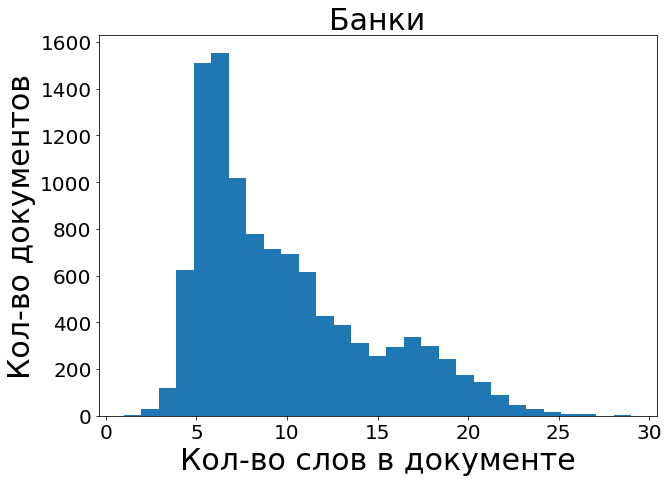
\includegraphics[width=0.5\textwidth]{images/hist_bank.png}
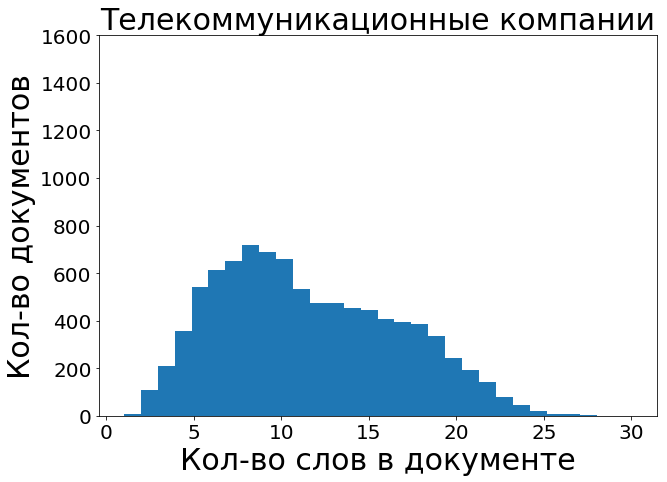
\includegraphics[width=0.5\textwidth]{images/hist_tkk.png}
\label{fig:hist_twitter}
\end{figure}
%--------------------------------------------------------------------------------
\section{Отзывы на товары и рестораны}
Данная выборка содержит отзывы на товары с ресурса \url{www.torg.mail.ru} и отзывы на рестораны с ресурса \url{www.restoclub.ru}.

Особенности:
\begin{itemize}
	\item Размер выборки - около 70 тыс. экземпляров
	\item Максимальная длина документа - 150 слов
	\item Средняя длина документа - 60 слов
\end{itemize}

Таблица \ref{tab:reviews} содержит статистику по числу экземпляров с определенной меткой. Рисунок \ref{fig:hist_reviews} содержит гистограмму с распределением длины документа для данной выборки.

\begin{table}[H]
\centering
\caption{Статистика по выборке с отзывами}
\label{tab:reviews}
\begin{tabular}{|c|c|c|c|}
\hline
\multirow{2}{*}{Подвыборка} & \multicolumn{3}{c|}{Документы}  \\ \cline{2-4} 
                            & Позитивные & Негативные & Сумма \\ \hline
Обучающая                   & 46925        & 12207       & 59132 \\ \hline
Тестовая                    & 11734        & 3050        & 14784  \\ \hline
\end{tabular}
\end{table}

\begin{figure}[H]
\centering
\caption{Распределение кол-ва слов в документе для выборки с отзывами}
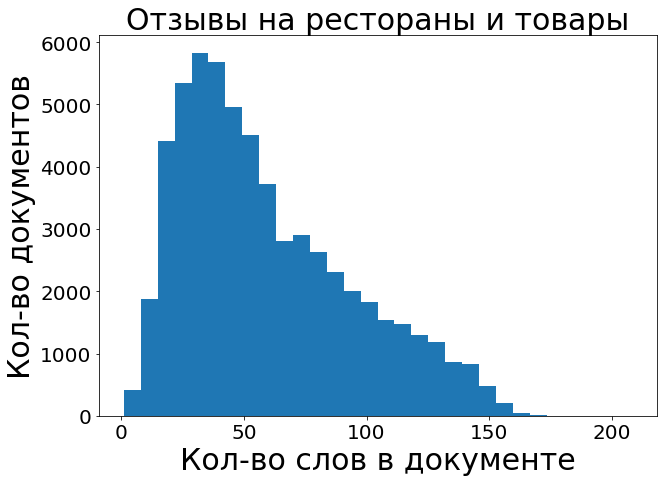
\includegraphics[width=0.5\textwidth]{images/hist_reviews.png}
\label{fig:hist_reviews}
\end{figure}
%--------------------------------------------------------------------------------
\section{Рецензии на фильмы}
Данная выборка содержит рецензии на 350 фильмов с ресурса \url{www.kinopoisk.ru}.

Особенности:
\begin{itemize}
	\item Размер выборки - около 30 тыс. экземпляров
	\item Максимальная длина документа - 1000 слов
	\item Средняя длина документа - 290 слов
\end{itemize}

Таблица \ref{tab:kinopoisk} содержит статистику по числу экземпляров с определенной меткой. Рисунок \ref{fig:hist_kinopoisk} содержит гистограмму с распределением длины документа для данной выборки.

\begin{table}[H]
\centering
\caption{Статистика по выборке с рецензиями}
\label{tab:kinopoisk}
\begin{tabular}{|c|c|c|c|c|}
\hline
\multirow{2}{*}{Подвыборка} & \multicolumn{4}{c|}{Документы}                \\ \cline{2-5} 
                            & Позитивные & Нейтральные & Негативные & Сумма \\ \hline
Обучающая                   & 21695        & 3627        & 3754       & 29076 \\ \hline
Тестовая                    & 5349        & 932        & 989        & 7270  \\ \hline
\end{tabular}
\end{table}

\begin{figure}[H]
\centering
\caption{Распределение кол-ва слов в документе для выборки с рецензиями}
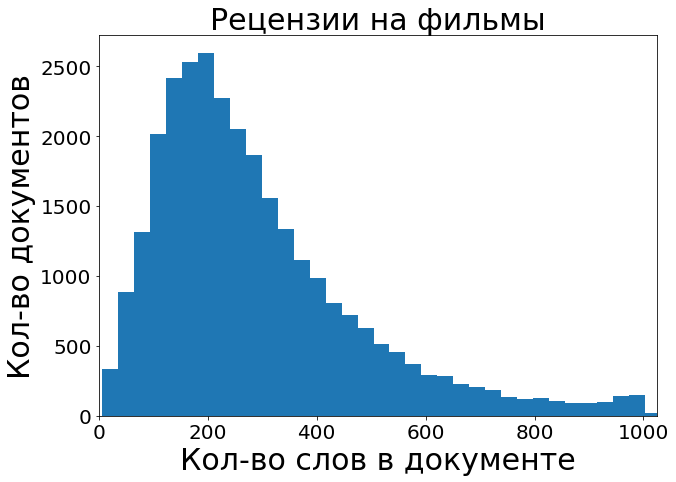
\includegraphics[width=0.5\textwidth]{images/hist_kinopoisk.png}
\label{fig:hist_kinopoisk}
\end{figure}           % Глава 2
\chapter{Описание предложенного алгоритма}

\section{Предобработка текста}
Предварительная предобработка текста состоит из следующих этапов:

\begin{enumerate}
	\item Токенизация текста - из документа (сообщения/отзыва) получаем последовательность слов (токенов). Осуществляется посредством библиотеки \texttt{NLTK}\footnote{https://www.nltk.org/}.
	\item Лемматизация слов - приведение слов к их леммам для сокращения словаря. Осуществляется посредством библиотеки \texttt{PyMorphy2}\footnote{https://pymorphy2.readthedocs.io/}.
	\item Векторизация слов - сопоставления словам плотных векторов фиксированной размерности. Используется предобученный на русскоязычном корпусе из социальных медиа \texttt{Word2Vec}\footnote{http://mlcourse.at.ispras.ru/}. Векторное пространство слов имеет размерность 300.
	\item Zero-padding - дополнение последовательностей векторов нулевыми векторами до заданной максимальной длины последовательности, зависящей от выборки.
\end{enumerate}

Полученное представление документа в виде последовательности слов-векторов будет далее подаваться на вход рекуррентной нейронной сети.

%-----------------------------------------------------
\section{Рекуррентная нейронная сеть}
Ключевой компонентой алгоритма решения поставленной задачи является однослойная двунаправленная рекуррентная нейронная сеть~\cite{schuster} типа GRU~\cite{cho}. GRU (Gated Recurrent Unit) может быть описан следующими уравнениями:
	\begin{align}
	z_{t}&=\sigma_{g}(W_{z}x_{t}+U_{z}h_{t-1})\\
	r_{t}&=\sigma_{g}(W_{r}x_{t}+U_{r}h_{t-1})\\
	\tilde{h}_{t}&=\tanh(Wx_{t}+U(r_{t}\circ h_{t-1}))\\
	h_{t}&=(1-z_{t})\circ \tilde{h}_{t}+z_{t}\circ h_{t-1}
	\end{align}	
где $x_{t}$ -- t-ый элемент последовательности, а $h_{t}$ -- внутреннее состояние сети в t-ый момент времени (после обработки $x_{t}$).

Входная последовательность подается на вход одной рекуррентной сети прямым порядком и другой сети - обратным. После чего выходы этих двух слоёв конкатенируются, образуя выходную последовательность $y_{t} = \left[\overrightarrow{h_{t}},\overleftarrow{h_{t}}\right]$. Таким образом строится двунаправленная рекуррентная сеть, архитектура которой изображена на Рисунке~\ref{fig:birnn}.

\begin{figure}[H]
  \centering
  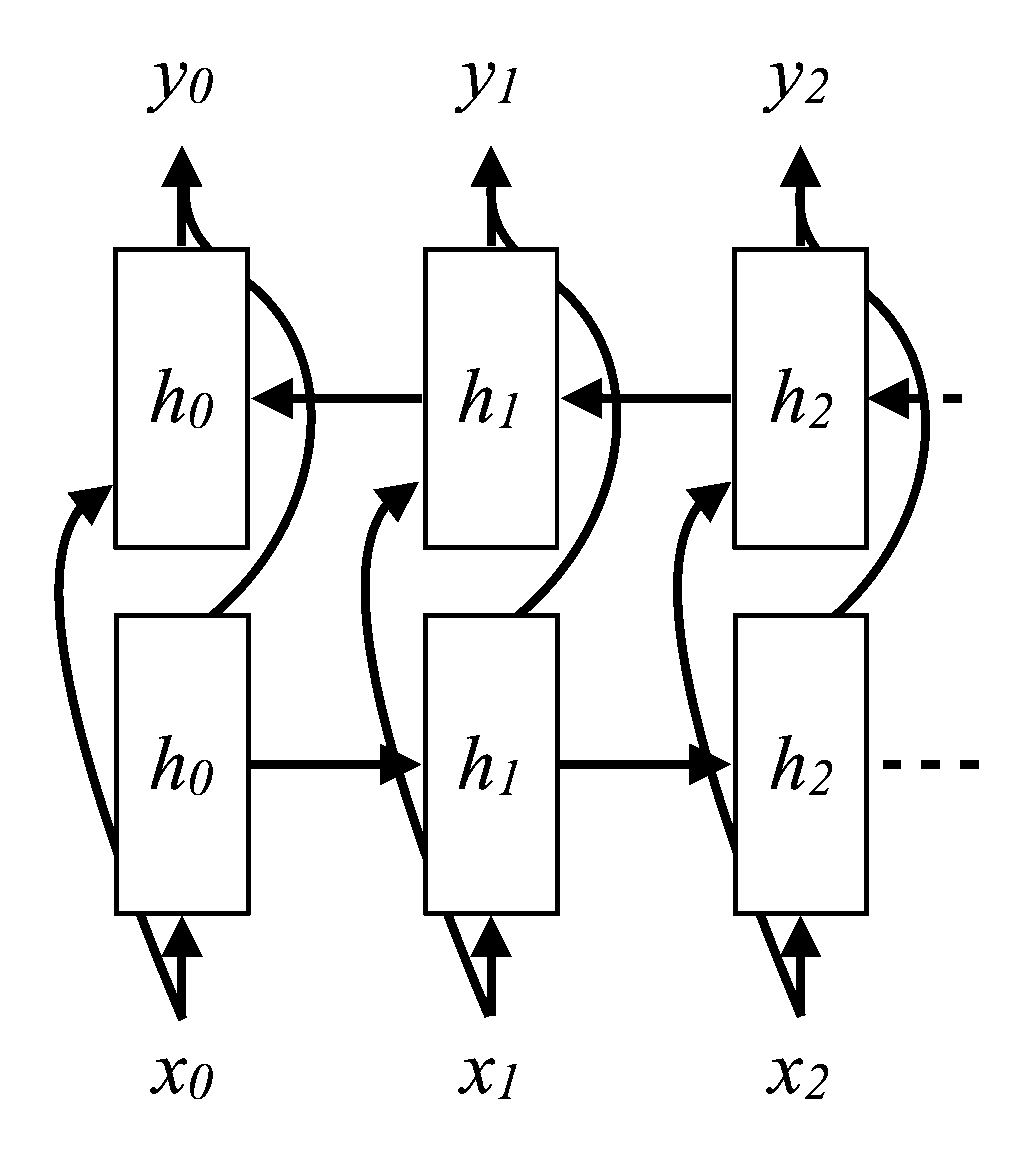
\includegraphics[width=0.5\textwidth]{images/birnn2_bin.png}
  \caption{Двунаправленная рекуррентная нейронная сеть}
  \label{fig:birnn}
\end{figure}
%-----------------------------------------------------
\section{Механизм внимания}
Классическим подходом к работе с выходом рекуррентной нейронной сети - $y_{1} ,..., y_{T} $ является рассмотрение лишь последнего вектора $y_{T}$, где $T$ -- длина входной (и выходной) последовательности, т.к. он аккумулирует в себе извлеченную информацию из всей входной последовательности. Рассматриваемый же нами подход -- механизм внимания~\cite{bahdanau} -- утилизирует все выходные векторы $y_{t}$, вычисляя их линейную комбинацию с коэффициентами $\alpha_{t}$, которые обучаются вместе с остальной сетью. Уравнения механизма внимания выглядят следующим образом:
	\begin{align}	
    \upsilon_{t}&=\tanh{(W_{\omega}y_{t}+b_{\omega})}\\
	\alpha_{t}&=\frac{\exp{(\upsilon_{t}^{T}u_{\omega})}}{\sum_{j=1}^{T}\exp{(\upsilon_{j}^{T}u_{\omega})}}\\
	\upsilon&=\sum_{t=1}^{T}\alpha_{t}y_{t}
	\end{align}	
Архитектура двунаправленной рекуррентной нейронной сети с механизмом внимания представлена на Рис.~\ref{fig:att}. Во время обучения к выходу слоя механизма внимания $\upsilon$ применяется регуляризатор Dropout~\cite{srivastava} для уменьшения переобучения.

\begin{figure}[H]
  \centering
  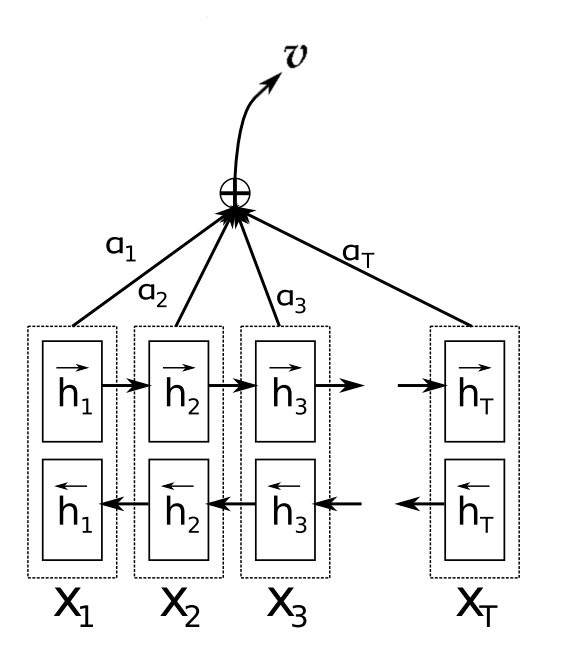
\includegraphics[width=0.5\textwidth]{images/att_edited.png}
  \caption{Двунаправленная рекуррентная нейронная сеть с механизмом внимания}
  \label{fig:att}
\end{figure}
%-----------------------------------------------------
\section{Полносвязанный слой}
После слоя механизма внимания следует полносвязный слой с функцией активации $softmax$, переводящий вектор $\upsilon$ в двух или трёхмерное пространство (в зависимости от числа классов в выборке), где каждое из чисел обозначает вероятность принадлежности объекта к соответствующему классу:
	\begin{align}	
    \hat{s}&=(\hat{s}^{(-1)},\hat{s}^{(0)},\hat{s}^{(1)})=softmax(W\upsilon+b)
	\end{align}
%-----------------------------------------------------
\section{Обучение}
Классификатор обучается при помощи метода оптимизации Adam и обратного распространения, минимизируя перекрёстную энтропию между выходным распределением $\hat{s}$ и истинным $s$:
    \begin{align}
    L(W)=-\sum_{i=1}^{n}\sum_{c\in\left \{ -1,0,1 \right \}}s_{i}^{(c)}\log{\hat{s_{i}}^{(c)}},
    \end{align}
Параметры модели подбираются по сетке при помощи перекрёстной валидации.
           % Глава 3
\chapter{Вычислительный эксперимент}

\section{Твиты}
В Таблице \ref{tab:res_twitter} представлены результаты 5-фолд кросс-валидации различных моделей на обучающей подвыборке и результаты на тестовой подвыборке для набора с твитами. Используемая метрика - макро-усреднённая F1-мера по классам положительной и отрицательной тональностей. Помимо наших экспериментов в таблице представлены результаты победителя~\cite{arhipenko}  и бейзлайны соревновательной дорожки по анализу тональности Dialogue Evaluate 2016~\cite{senti-ru-eval}. Здесь стоит отметить, что решения участников соревнования содержали различные дополнительные методы обработки данных, такие как, например, удаление полудубликатов из обучающей выборки.

Видно, что лишь на одном из двух доменов алгоритм с исследуемым механизмом внимания превзошёл аналогичный алгоритм без механизма внимания.

\begin{table}[H]
\centering
\caption{F1-мера различных моделей на кросс-валидации (CV) и на тестовой выборке}
\label{tab:res_twitter}
    \begin{tabular}{l|l|l|l|l|}
    \cline{2-5}
                                                                                                                  & \multicolumn{2}{c|}{Banks}   & \multicolumn{2}{c|}{\begin{tabular}[c]{@{}c@{}}Telecommunication\\ companies\end{tabular}} \\ \cline{2-5}                                                                                                               
                                                                                                                  & \begin{tabular}[c]{@{}l@{}}5-fold CV\\(mean, std)\end{tabular}  & test & \begin{tabular}[c]{@{}l@{}}5-fold CV\\(mean, std)\end{tabular}                                & test                                \\ \hline
    \multicolumn{1}{|l|}{Bi-GRU}                                                                                  & 0.74, 0.02            & 0.48 & 0.62, 0.01                                                     & 0.52                                \\ \hline
    \multicolumn{1}{|l|}{Bi-GRU + Attention}                                                                      & 0.74, 0.02            & 0.51 & 0.60, 0.02                                           & 0.49                                \\ \hline
    \multicolumn{1}{|l|}{\begin{tabular}[c]{@{}l@{}}2-layer GRU,\\ reversed sequences\\ (Arhipenko)\end{tabular}} & 0.62, -               & 0.55 & \textbf{0.66}, -                                              & \textbf{0.56}                                \\ \hline
    \multicolumn{1}{|l|}{Bi-GRU (Arhipenko)}                                                                      & 0.62, -               & -    & 0.65, -                                              & -                                   \\ \hline
    \multicolumn{1}{|l|}{LSTM (Arhipenko)}                                                                        & 0.60, -               & -    & 0.64, -                                              & -                                   \\ \hline
    \multicolumn{1}{|l|}{CNN (Arhipenko)}                                                                         & -                     & 0.48 & -                                                    & 0.47                                \\ \hline
    \multicolumn{1}{|l|}{SVM baseline}                                                                            & -                     & 0.46 & -                                                    & 0.46                                \\ \hline
    \multicolumn{1}{|l|}{Majority baseline}                                                                       & -                     & 0.31 & -                                                    & 0.19                                \\ \hline
    \end{tabular}
\end{table}

Также из таблицы видно, что значения F1-меры на обучающей и тестовой выборке существенно отличаются. Мы провели ряд экспериментов, для того чтобы найти гиперпараметры, при которых бы удалось уменьшить переобучение алгоритмов. Однако эта разница наблюдалась во всех наших экспериментах, как при уменьшении размера сети, так и с увеличением параметра регуляризации dropout~\cite{srivastava}. Чтобы исследовать причины этого расхождения, мы провели эксперимент со смешиванием обучающей и тестовой выборок и последующей кросс-валидацией моделей на смешанной выборке. Результаты данного эксперимента приведены в Таблице \ref{tab:mix}. Стоит отметить, что размеры обучающей и тестовой выборок сравнимы (5:2). Судя по тому, что кросс-валидация на смешанной выборке показала результаты очень близкие к кросс-валидации на обучающей выборке, можно предположить, что между обучающей и тестовой выборками есть существенные различия. Однако для тщательной проверки этой гипотезы требуется провести детальный сравнительный анализ данных, что авторы планируют проделать в будущем.

\begin{table}[H]
\centering
\caption{Результаты эксперимента со смешиванием обучающей и тестовой выборок, метрика - F1}
\label{tab:mix}
{\setlength{\tabcolsep}{0.25em}
\begin{tabular}{l|c|l|l|c|l|l|}
\cline{2-7}
                                         & \multicolumn{3}{c|}{Banks}                                                                                     & \multicolumn{3}{c|}{\begin{tabular}[c]{@{}c@{}}Telecommunication\\ companies\end{tabular}}                     \\ \cline{2-7} 
                                         & \multicolumn{2}{c|}{cross-validation}                             & \multicolumn{1}{c|}{\multirow{2}{*}{test}} & \multicolumn{2}{c|}{cross-validation}                             & \multicolumn{1}{c|}{\multirow{2}{*}{test}} \\ \cline{2-3} \cline{5-6}
                                         & train                           & \multicolumn{1}{c|}{train+test} & \multicolumn{1}{c|}{}                      & train                           & \multicolumn{1}{c|}{train+test} & \multicolumn{1}{c|}{}                      \\ \hline
\multicolumn{1}{|l|}{Bi-GRU}             & \multicolumn{1}{l|}{0.74, 0.02} & 0.71, 0.02                      & 0.48                                       & \multicolumn{1}{l|}{0.62, 0.01} & 0.62, 0.01                      & 0.52                                       \\ \hline
\multicolumn{1}{|l|}{Bi-GRU+Attention} & \multicolumn{1}{l|}{0.74, 0.02} & 0.72, 0.01                      & 0.51                                       & \multicolumn{1}{l|}{0.60, 0.02} & 0.62, 0.01                      & 0.49                                       \\ \hline
\end{tabular}}
\end{table}

%------------------------------------------------------------------------------
\section{Отзывы на товары и рестораны}
В Таблице \ref{tab:res_reviews} представлены результаты 10-фолд кросс-валидации различных моделей на обучающей подвыборке и результаты на тестовой подвыборке для набора отзывов на товары и рестораны. Используемые метрики - точность (accuracy) и макро-усреднённая F1-мера по классам положительной и отрицательной тональностей.

\begin{table}[H]
	\centering
	\caption{Качество различных моделей на кросс-валидации (CV) и тестовой подвыборке для набора с отзывами}
	\label{tab:res_reviews}
	\begin{tabular}{l|l|l|l|l|}
		\cline{2-5}
		& \multicolumn{4}{c|}{Reviews}                                                                                      \\ \cline{2-5} 
		& \multicolumn{2}{c|}{10-fold CV}                         & \multicolumn{2}{c|}{test}                               \\ \cline{2-5} 
		& \multicolumn{1}{c|}{accuracy} & \multicolumn{1}{c|}{F1} & \multicolumn{1}{c|}{accuracy} & \multicolumn{1}{c|}{F1} \\ \hline
		\multicolumn{1}{|l|}{Bi-GRU}           & 0.906, 0.003                  & 0.863, 0.007            & \textbf{0.901}                         & \textbf{0.861}                   \\ \hline
		\multicolumn{1}{|l|}{Bi-GRU+Attention} & 0.907, 0.004                  & 0.865, 0.007            & 0.900                         & \textbf{0.861}                   \\ \hline
		\multicolumn{1}{|l|}{CNN}              & 0.901, 0.003                  & 0.854, 0.005            & 0.896                         & 0.844                   \\ \hline
		\multicolumn{1}{|l|}{SVM}              & 0.897, 0.004                  & 0.838, 0.006            & 0.895                         & 0.836                   \\ \hline
		\multicolumn{1}{|l|}{Majority baseline}              & -                  & -            & 0.793                         & 0.442                   \\ \hline
	\end{tabular}
\end{table}

Как видно из таблицы, в эксперименте с отзывами предложенный алгоритм также не превзошёл двунаправленную рекуррентную нейронную сеть.

%------------------------------------------------------------------------------
\section{Рецензии на фильмы}
В Таблице \ref{tab:res_kinopoisk} представлены результаты 10-фолд кросс-валидации различных моделей на обучающей подвыборке и результаты на тестовой подвыборке для набора рецензий на фильмы. Используемые метрики - точность (accuracy) и макро-усреднённая F1-мера по всем трём классам.

\begin{table}[H]
	\centering
	\caption{Качество различных моделей на кросс-валидации (CV) и тестовой подвыборке для набора с рецензиями}
	\label{tab:res_kinopoisk}
	\begin{tabular}{l|l|l|l|l|}
        \cline{2-5}
                                                & \multicolumn{4}{c|}{Reviews}                                                                                      \\ \cline{2-5} 
                                                & \multicolumn{2}{c|}{10-fold CV}                         & \multicolumn{2}{c|}{test}                               \\ \cline{2-5} 
                                                & \multicolumn{1}{c|}{Accuracy} & \multicolumn{1}{c|}{F1} & \multicolumn{1}{c|}{Accuracy} & \multicolumn{1}{c|}{F1} \\ \hline
        \multicolumn{1}{|l|}{Bi-GRU}            & 0.833, 0.004                  & 0.647, 0.005            & 0.807                         & 0.640                   \\ \hline
        \multicolumn{1}{|l|}{Bi-GRU+Attention}  & 0.837, 0.004                  & 0.655, 0.006            & \textbf{0.811}                         & \textbf{0.648}                   \\ \hline
        \multicolumn{1}{|l|}{CNN}               & 0.821, 0.005                  & 0.649, 0.005            & 0.775                         & 0.637                   \\ \hline
        \multicolumn{1}{|l|}{SVM}               & 0.824, 0.003                  & 0.541, 0.003            & 0.798                         & 0.375                   \\ \hline
        \multicolumn{1}{|l|}{Majority baseline} & -                             & -                       & 0.735                         & 0.282                   \\ \hline
    \end{tabular}
\end{table}

В эксперименте с выборкой, состоящей из наиболее крупных документов - рецензий, предложенный алгоритм превзошёл остальные алгоритмы как на валидации, так и на тестовой подвыборке. Данный результат можно объяснить тем, что рекуррентные нейронные сети имеют свойство терять информацию из середины входной последовательности в случае достаточно длинного входа, и с данной проблемой должна помочь некоторая аггрегация скрытых состояний рекуррентного слоя, что и происходит в механизме внимания.
           % Глава 4
\chapter{Заключение}

Таким образом, исследована применимость модели на основе двунаправленной рекуррентной нейронной сети с механизмом внимания в задаче классификации тональности русскоязычных текстов. Проведён подбор гиперпараметров и обучены модели на нескольких наборах данных. Проведено сравнение данной модели с её ранее изученными аналогами. Выявлено преимущество использования предложенной архитектуры в случае достаточно длинных документов (порядка 300 слов), а именно, для рецензий на фильмы с ресурса \url{www.kinopoisk.ru}.

В рамках данной работы реализован алгоритм двунаправленной рекуррентной нейронной сети с механизмом внимания. Код отлажен и выложен в открытый доступ \url{www.github.com/ilivans/tf-rnn-attention}. Также доступен весь код, использованный в работе, значения гиперпараметров моделей и сам отчёт \url{www.github.com/ilivans/attention-sentiment}.

Для дальнейшего исследования предлагается изучить применимость более сложных и глубоких архитектур для анализа тональности русскоязычных текстов, а также применимость данной модели в качестве модуля для нейронной сети, генерирующей сообщения с заданной тональностью.
           % Глава 5
% \chapter*{Заключение}						% Заголовок
\addcontentsline{toc}{chapter}{Заключение}	% Добавляем его в оглавление

%% Согласно ГОСТ Р 7.0.11-2011:
%% 5.3.3 В заключении диссертации излагают итоги выполненного исследования, рекомендации, перспективы дальнейшей разработки темы.
%% 9.2.3 В заключении автореферата диссертации излагают итоги данного исследования, рекомендации и перспективы дальнейшей разработки темы.
%% Поэтому имеет смысл сделать эту часть общей и загрузить из одного файла в автореферат и в диссертацию:

Основные результаты работы заключаются в следующем.
%% Согласно ГОСТ Р 7.0.11-2011:
%% 5.3.3 В заключении диссертации излагают итоги выполненного исследования, рекомендации, перспективы дальнейшей разработки темы.
%% 9.2.3 В заключении автореферата диссертации излагают итоги данного исследования, рекомендации и перспективы дальнейшей разработки темы.
\begin{enumerate}
  \item На основе анализа \ldots
  \item Численные исследования показали, что \ldots
  \item Математическое моделирование показало \ldots
  \item Для выполнения поставленных задач был создан \ldots
\end{enumerate}

И какая-нибудь заключающая фраза.

Последний параграф может включать благодарности.  В заключение автор
выражает благодарность и большую признательность научному руководителю
Иванову~И.И. за поддержку, помощь, обсуждение результатов и научное
руководство. Также автор благодарит Сидорова~А.А. и Петрова~Б.Б. за
помощь в работе с образцами, Рабиновича~В.В. за предоставленные
образцы и обсуждение результатов, Занудятину~Г.Г. и авторов шаблона
*Russian-Phd-LaTeX-Dissertation-Template* за помощь в оформлении
диссертации. Автор также благодарит много разных людей и
всех, кто сделал настоящую работу автора возможной.
      % Заключение
% \chapter*{Список сокращений и условных обозначений}             % Заголовок
\addcontentsline{toc}{chapter}{Список сокращений и условных обозначений}  % Добавляем его в оглавление
\noindent
\addtocounter{table}{-1}% Нужно откатить на единицу счетчик номеров таблиц, так как следующая таблица сделана для удобства представления информации по ГОСТ
%\begin{longtabu} to \dimexpr \textwidth-5\tabcolsep {r X}
\begin{longtabu} to \textwidth {r X}
% Жирное начертание для математических символов может иметь
% дополнительный смысл, поэтому они приводятся как в тексте
% диссертации
$\begin{rcases}
a_n\\
b_n
\end{rcases}$  & 
\begin{minipage}{\linewidth}
коэффициенты разложения Ми в дальнем поле соответствующие
электрическим и магнитным мультиполям
\end{minipage}
\\
${\boldsymbol{\hat{\mathrm e}}}$ & единичный вектор \\
$E_0$ & амплитуда падающего поля\\
$\begin{rcases}
a_n\\
b_n
\end{rcases}$  & 
коэффициенты разложения Ми в дальнем поле соответствующие
электрическим и магнитным мультиполям ещё раз, но без окружения
minipage нет вертикального выравнивания по центру.
\\
$j$ & тип функции Бесселя\\
$k$ & волновой вектор падающей волны\\

$\begin{rcases}
a_n\\
b_n
\end{rcases}$  & 
\begin{minipage}{\linewidth}
\vspace{0.7em}
и снова коэффициенты разложения Ми в дальнем поле соответствующие
электрическим и магнитным мультиполям, теперь окружение minipage есть
и добавленно много текста, так что описание группы условных
обозначений значительно превысило высоту этой группы... Для отбивки
пришлось добавить дополнительные отступы.
\vspace{0.5em}
\end{minipage}
\\
$L$ & общее число слоёв\\
$l$ & номер слоя внутри стратифицированной сферы\\
$\lambda$ & длина волны электромагнитного излучения
в вакууме\\
$n$ & порядок мультиполя\\
$\begin{rcases}
{\mathbf{N}}_{e1n}^{(j)}&{\mathbf{N}}_{o1n}^{(j)}\\
{\mathbf{M}_{o1n}^{(j)}}&{\mathbf{M}_{e1n}^{(j)}}
\end{rcases}$  & сферические векторные гармоники\\
$\mu$  & магнитная проницаемость в вакууме\\
$r,\theta,\phi$ & полярные координаты\\
$\omega$ & частота падающей волны\\

  \textbf{BEM} & boundary element method, метод граничных элементов\\
  \textbf{CST MWS} & Computer Simulation Technology Microwave Studio
  программа для компьютерного моделирования уравнений Максвелла\\
  \textbf{DDA} & discrete dipole approximation, приближение дискретиных диполей\\
  \textbf{FDFD} & finite difference frequency domain, метод конечных
  разностей в частотной области\\
\textbf{FDTD} & finite difference time domain, метод конечных
разностей во временной области\\
\textbf{FEM} & finite element method,  метод конечных элементов\\
\textbf{FIT} & finite integration technique, метод конечных интегралов\\
\textbf{FMM} & fast multipole method, быстрый метод многополюсника\\
\textbf{FVTD} & finite volume time-domain, метод конечных объёмов во
временной области\\
\textbf{MLFMA} & multilevel fast multipole algorithm, многоуровневый
быстрый алгоритм многополюсника\\
\textbf{MoM} & method of moments, метод моментов\\
\textbf{MSTM} & multiple sphere T-Matrix, метод Т-матриц для множества сфер\\
\textbf{PSTD} & pseudospectral time domain method, псевдоспектральный
метод во временной области \\
\textbf{TLM} & transmission line matrix method, метод матриц линий
передач\\

\end{longtabu}
        % Список сокращений и условных обозначений
% \chapter*{Словарь терминов}             % Заголовок
\addcontentsline{toc}{chapter}{Словарь терминов}  % Добавляем его в оглавление

\textbf{TeX} - Cистема компьютерной вёрстки, разработанная американским профессором информатики Дональдом Кнутом

\textbf{Панграмма} - Короткий текст, использующий все или почти все буквы алфавита
      % Словарь терминов
\clearpage                                  % В том числе гарантирует, что список литературы в оглавлении будет с правильным номером страницы
\phantomsection
\addcontentsline{toc}{chapter}{\bibname}	% Добавляем список литературы в оглавление
%\hypersetup{ urlcolor=black }               % Ссылки делаем чёрными
%\providecommand*{\BibDash}{}                % В стилях ugost2008 отключаем использование тире как разделителя 
\urlstyle{rm}                               % ссылки URL обычным шрифтом
\insertbibliofull                          % Подключаем Bib-базы
\urlstyle{tt}                               % возвращаем установки шрифта ссылок URL
%\hypersetup{ urlcolor={urlcolor} }          % Восстанавливаем цвет ссылок      % Список литературы
% \clearpage
\phantomsection
\addcontentsline{toc}{chapter}{\listfigurename}
\listoffigures									% Список изображений


%%% Список таблиц %%%
% (ГОСТ Р 7.0.11-2011, 5.3.10)
\clearpage
\phantomsection
\addcontentsline{toc}{chapter}{\listtablename}
\listoftables									% Список таблиц
\newpage           % Списки таблиц и изображений (иллюстративный материал)
\appendix
%% Правка оформления ссылок на приложения:
%http://tex.stackexchange.com/questions/56839/chaptername-is-used-even-for-appendix-chapters-in-toc
%http://tex.stackexchange.com/questions/59349/table-of-contents-with-chapter-and-appendix
%% требует двойной компиляции
\addtocontents{toc}{\def\protect\cftchappresnum{\appendixname{} }%
\setlength{\cftchapnumwidth}{\widthof{\cftchapfont\appendixname~Ш\cftchapaftersnum}}%
}
%% Оформление заголовков приложений ближе к ГОСТ:
\sectionformat{\chapter}[display]{% Параметры заголовков разделов в тексте
    label=\chaptertitlename\ \thechapter,% (ГОСТ Р 2.105, 4.3.6)
    labelsep=20pt,
}
\renewcommand\thechapter{\Asbuk{chapter}} % Чтобы приложения русскими буквами нумеровались
   % Предварительные настройки для правильного подключения Приложений
\chapter{Визуализированные примеры распределения весов слоя механизма внимания} \label{visual}
В данном приложении продемонстрированы примеры документов из тестовых подвыборок (неучаствовавших в обучении), которые были пропущены через обученную модель. Интенсивностью фонового цвета изображён вес $\alpha_{t}$ (чем интенсивнее, тем больше) при векторе, соответствующем данному слову $x_{t}$. Как можно видеть, механизм внимания действительно 'обращает внимание' на значимые (сигнальные) слова и их окрестности, чему соответствует яркий фон под подобными словами.

\begin{enumerate}
    \item \colorbox{yellow!70}{Почему-то}
\colorbox{yellow!100}{не}
\colorbox{yellow!57}{приходят}
\colorbox{yellow!17}{смс-сообщения}
\colorbox{yellow!5}{для}
\colorbox{yellow!7}{подтверждения}
\colorbox{yellow!0}{входа}
    \item \colorbox{yellow!3}{IPhone-овское}
\colorbox{yellow!2}{приложение}
\colorbox{yellow!2}{от}
\colorbox{yellow!30}{Сбербанка}
\colorbox{yellow!89}{самое}
\colorbox{yellow!100}{удобное}
\colorbox{yellow!84}{в}
\colorbox{yellow!82}{России}
    \item \colorbox{yellow!14}{Заведение}
\colorbox{yellow!41}{вполне}
\colorbox{yellow!62}{приличное,}
\colorbox{yellow!78}{кухня}
\colorbox{yellow!99}{хорошая,}
\colorbox{yellow!27}{но}
\colorbox{yellow!25}{маловато}
\colorbox{yellow!11}{выбора,}
\colorbox{yellow!8}{зато}
\colorbox{yellow!2}{с}
\colorbox{yellow!2}{напитками}
\colorbox{yellow!2}{никакой}
\colorbox{yellow!2}{проблемы}
\colorbox{yellow!3}{выбора}
\colorbox{yellow!2}{нет!!}
\colorbox{yellow!2}{много}
\colorbox{yellow!2}{сортов}
\colorbox{yellow!2}{пива}
\colorbox{yellow!3}{и}
\colorbox{yellow!2}{других}
\colorbox{yellow!1}{более}
\colorbox{yellow!2}{крепких}
\colorbox{yellow!1}{напитков.}
\colorbox{yellow!1}{из}
\colorbox{yellow!3}{минусов}
\colorbox{yellow!3}{можно}
\colorbox{yellow!4}{сказать}
\colorbox{yellow!4}{только}
\colorbox{yellow!10}{черезмерная}
\colorbox{yellow!8}{громкость}
\colorbox{yellow!12}{живой}
\colorbox{yellow!8}{музыки}
\colorbox{yellow!4}{по}
\colorbox{yellow!5}{выходным.}
\colorbox{yellow!6}{соседа}
\colorbox{yellow!11}{не}
\colorbox{yellow!11}{слышно....}
    \item \colorbox{yellow!4}{Нолан}
\colorbox{yellow!0}{—}    
\colorbox{yellow!6}{мой}
\colorbox{yellow!6}{любимый}
\colorbox{yellow!8}{режиссер.}
\colorbox{yellow!3}{А}
\colorbox{yellow!4}{его}
\colorbox{yellow!3}{«Помни»}
\colorbox{yellow!0}{—}
\colorbox{yellow!4}{мой}
\colorbox{yellow!4}{любимый}
\colorbox{yellow!4}{фильм.}
\colorbox{yellow!2}{Но}
\colorbox{yellow!1}{только}
\colorbox{yellow!0}{сейчас}
\colorbox{yellow!0}{я}
\colorbox{yellow!1}{с}
\colorbox{yellow!3}{удивлением}
\colorbox{yellow!2}{узнала,}
\colorbox{yellow!2}{что}
\colorbox{yellow!4}{«Престиж»}
\colorbox{yellow!1}{снял}
\colorbox{yellow!2}{тот}
\colorbox{yellow!2}{же}
\colorbox{yellow!7}{режиссер.}
\colorbox{yellow!5}{Собственно,}
\colorbox{yellow!6}{сам}
\colorbox{yellow!11}{фильм}
\colorbox{yellow!2}{я}
\colorbox{yellow!0}{посмотрела}
\colorbox{yellow!2}{не}
\colorbox{yellow!3}{из-за}
\colorbox{yellow!3}{громких}
\colorbox{yellow!3}{имен}
\colorbox{yellow!5}{актеров}
\colorbox{yellow!2}{и}
\colorbox{yellow!6}{режиссера,}
\colorbox{yellow!3}{а}
\colorbox{yellow!3}{потому,}
\colorbox{yellow!3}{что}
\colorbox{yellow!3}{прочитала}
\colorbox{yellow!4}{книгу.}
\colorbox{yellow!4}{Произведение}
\colorbox{yellow!3}{Кристофера}
\colorbox{yellow!3}{Приста}
\colorbox{yellow!5}{словно}
\colorbox{yellow!5}{схватило}
\colorbox{yellow!3}{меня}
\colorbox{yellow!3}{за}
\colorbox{yellow!5}{душу}
\colorbox{yellow!2}{и}
\colorbox{yellow!3}{не}
\colorbox{yellow!5}{отпускало}
\colorbox{yellow!2}{до}
\colorbox{yellow!2}{самого}
\colorbox{yellow!4}{конца.}
\colorbox{yellow!3}{А}
\colorbox{yellow!2}{вечером}
\colorbox{yellow!3}{я}
\colorbox{yellow!13}{пересказывала}
\colorbox{yellow!39}{историю}
\colorbox{yellow!7}{двух}
\colorbox{yellow!20}{иллюзионистов}
\colorbox{yellow!3}{своей}
\colorbox{yellow!2}{подруге,}
\colorbox{yellow!1}{которая}
\colorbox{yellow!3}{понимала}
\colorbox{yellow!2}{меня}
\colorbox{yellow!2}{с}
\colorbox{yellow!2}{трудом,}
\colorbox{yellow!2}{ведь}
\colorbox{yellow!2}{сам}
\colorbox{yellow!6}{сюжет}
\colorbox{yellow!8}{настолько}
\colorbox{yellow!11}{лихо}
\colorbox{yellow!26}{закручен,}
\colorbox{yellow!13}{а}
\colorbox{yellow!10}{конец}
\colorbox{yellow!12}{просто}
\colorbox{yellow!16}{шедеврален!}
\colorbox{yellow!23}{И}
\colorbox{yellow!9}{на}
\colorbox{yellow!9}{этой}
\colorbox{yellow!55}{позитивной}
\colorbox{yellow!56}{ноте}
\colorbox{yellow!38}{я}
\colorbox{yellow!32}{взялась}
\colorbox{yellow!19}{за}
\colorbox{yellow!16}{фильм.}
\colorbox{yellow!11}{Скажу}
\colorbox{yellow!20}{честно}
\colorbox{yellow!0}{—}
\colorbox{yellow!49}{разочаровал.}
\colorbox{yellow!54}{Скучнее}
\colorbox{yellow!65}{я}
\colorbox{yellow!30}{ничего}
\colorbox{yellow!13}{не}
\colorbox{yellow!47}{видела.}
\colorbox{yellow!9}{После}
\colorbox{yellow!6}{нескольких}
\colorbox{yellow!7}{первых}
\colorbox{yellow!5}{минут}
\colorbox{yellow!10}{я}
\colorbox{yellow!4}{начала}
\colorbox{yellow!3}{«пропадать»}
\colorbox{yellow!4}{в}
\colorbox{yellow!16}{сюжете.}
\colorbox{yellow!25}{Он}
\colorbox{yellow!41}{оказался}
\colorbox{yellow!53}{уж}
\colorbox{yellow!100}{больно}
\colorbox{yellow!41}{запутанным,}
\colorbox{yellow!27}{да}
\colorbox{yellow!13}{так,}
\colorbox{yellow!4}{что,}
\colorbox{yellow!18}{кажется,}
\colorbox{yellow!26}{сценарист}
\colorbox{yellow!18}{сам}
\colorbox{yellow!5}{в}
\colorbox{yellow!11}{нем}
\colorbox{yellow!30}{запутался}
\colorbox{yellow!34}{с}
\colorbox{yellow!45}{режиссером}
\colorbox{yellow!8}{на}
\colorbox{yellow!3}{пару.}
\colorbox{yellow!2}{Всё}
\colorbox{yellow!4}{время}
\colorbox{yellow!26}{пыталась}
\colorbox{yellow!14}{связать}
\colorbox{yellow!10}{происходящее}
\colorbox{yellow!4}{на}
\colorbox{yellow!5}{экране}
\colorbox{yellow!7}{с}
\colorbox{yellow!6}{книгой,}
\colorbox{yellow!13}{но,}
\colorbox{yellow!16}{как}
\colorbox{yellow!7}{ни}
\colorbox{yellow!34}{старалась,}
\colorbox{yellow!17}{ничего}
\colorbox{yellow!78}{общего}
\colorbox{yellow!25}{не}
\colorbox{yellow!16}{нашла.}
\colorbox{yellow!10}{Вкуснейшая}
\colorbox{yellow!32}{интрига}
\colorbox{yellow!5}{Приста}
\colorbox{yellow!5}{была}
\colorbox{yellow!13}{отвратительно}
\colorbox{yellow!14}{чем-то}
\colorbox{yellow!12}{разбавлена.}
\colorbox{yellow!29}{Блюдо}
\colorbox{yellow!41}{остыло}
\colorbox{yellow!8}{и}
\colorbox{yellow!6}{дорога}
\colorbox{yellow!6}{ему}
\colorbox{yellow!5}{на}
\colorbox{yellow!4}{помойку.}
\colorbox{yellow!4}{Единственное,}
\colorbox{yellow!4}{что}
\colorbox{yellow!5}{хоть}
\colorbox{yellow!10}{немного}
\colorbox{yellow!16}{меня}
\colorbox{yellow!16}{порадовало,}
\colorbox{yellow!12}{так}
\colorbox{yellow!11}{это}
\colorbox{yellow!30}{актерский}
\colorbox{yellow!7}{состав.}
\colorbox{yellow!19}{Игра}
\colorbox{yellow!18}{потрясающая,}
\colorbox{yellow!34}{но}
\colorbox{yellow!45}{со}
\colorbox{yellow!18}{Скарлетт}
\colorbox{yellow!4}{что-то}
\colorbox{yellow!3}{было}
\colorbox{yellow!2}{не}
\colorbox{yellow!3}{так.}
\colorbox{yellow!3}{Возможно,}
\colorbox{yellow!4}{дело}
\colorbox{yellow!2}{в}
\colorbox{yellow!4}{самой}
\colorbox{yellow!4}{Оливии.}
\colorbox{yellow!2}{Кажется,}
\colorbox{yellow!2}{в}
\colorbox{yellow!2}{книге}
\colorbox{yellow!2}{этот}
\colorbox{yellow!3}{персонаж}
\colorbox{yellow!1}{был}
\colorbox{yellow!0}{полнее.}
\colorbox{yellow!1}{В}
\colorbox{yellow!1}{общем,}
\colorbox{yellow!1}{в}
\colorbox{yellow!5}{попытке}
\colorbox{yellow!5}{переделать}
\colorbox{yellow!7}{роман}
\colorbox{yellow!2}{на}
\colorbox{yellow!2}{большой}
\colorbox{yellow!3}{экран,}
\colorbox{yellow!3}{была}
\colorbox{yellow!2}{уничтожена}
\colorbox{yellow!3}{вся}
\colorbox{yellow!7}{острота}
\colorbox{yellow!0}{начинки.}
\colorbox{yellow!0}{Для}
\colorbox{yellow!0}{меня,}
\colorbox{yellow!0}{это}
\colorbox{yellow!0}{—}
\colorbox{yellow!0}{худшая}
\colorbox{yellow!0}{экранизация}
\colorbox{yellow!0}{прочитанной}
\colorbox{yellow!0}{книги.}
\colorbox{yellow!0}{Вот}
\colorbox{yellow!0}{так}
\colorbox{yellow!0}{вот.}
\end{enumerate}
% 1.
% \colorbox{yellow!70}{Почему-то}
% \colorbox{yellow!100}{не}
% \colorbox{yellow!57}{приходят}
% \colorbox{yellow!17}{смс-сообщения}
% \colorbox{yellow!5}{для}
% \colorbox{yellow!7}{подтверждения}
% \colorbox{yellow!0}{входа}
% \linebreak
% 2.
% \colorbox{yellow!3}{IPhone-овское}
% \colorbox{yellow!2}{приложение}
% \colorbox{yellow!2}{от}
% \colorbox{yellow!30}{Сбербанка}
% \colorbox{yellow!89}{самое}
% \colorbox{yellow!100}{удобное}
% \colorbox{yellow!84}{в}
% \colorbox{yellow!82}{России}
% \linebreak        % Приложения

\end{document}
